
\chapter{O CERN e a Física Experimental de Altas Energias}
\label{cap:cern}
\glsresetall

O CERN é o maior laboratório de Física de Partículas do mundo situado na fronteira
entre a França e a Suíça, e conta com a colaboração de diversos países membros na
Europa e associados como Brasil e Estados Unidos. Desde sua fundação em 1954,
após a Segunda Guerra, tem sido uma das das maiores referências neste campo e um
dos maiores pólos de avanços tecnológicos do mundo. Dentre seus feitos constam a 
construção do primeiro colisor de prótons-prótons (1971), a descobertas dos  bósons 
Z e W (1983), a invenção da \emph{Web} (1990), e recentemente, a descoberta 
do bóson de Higgs em 2012, anunciada em conjunto
pelos dois maiores detectores de partículas do mundo instalados no \gls{cern}.

O propósito deste capítulo é descrever o ambiente no qual este trabalho está inserido. 
Primeiramente, daremos uma breve introdução à Física de partículas, ao \gls{mp}, 
o experimento  \gls{lhc} e os detectores nele instalados. Um foco maior será dado
ao detector \gls{atlas}, o ambiente deste trabalho, descrevendo seus sub-detectores
e seu sistema de filtragem online.

\section{O Modelo Padrão}

Qualquer teoria de Física de Partículas Elementares precisa ser consistente com
a Relatividade Especial. A junção da Mecânica Quântica, Eletromagnetismo e
Relatividade Especial foi realizada através da Teoria Quântica
dos Campos. A Teoria dos Campos teve como seu primeiro triunfo a
\gls{qed}, que descreve a interação de partículas carregadas com o campo
eletromagnético. 

O \gls{mp}, como o \gls{qed} nele contido, é uma teoria de interação de campos. 
Ele descreve de maneira bem sucedida as relações entre partículas elementares 
conhecidas pela ciência atual \cite{Intro_Nuclear} e as características de três 
interações entre essas partículas: eletromagnética, fraca e forte. A interação 
gravitacional é desprezível na escala da Física de Partículas, onde a massa da 
partículas é da ordem de $10^{-27}$~kg \cite{Intro_Standard}.

São utilizados no \gls{mp} doze férmions, partículas elementares, divididas em dois 
grupos: os léptons e os quarks. Existem três diferentes gerações, ou famílias, de férmions, 
cada uma com maior massa. Ainda, existem quatro outras partículas de campo das interações, 
chamadas de bósons de campo. A Figura~\ref{fig:modelo_padrao} contém as diferentes 
partículas que são descritas pelo \gls{mp}, e seus respectivos números quânticos, como as 
massas de repouso em $GeV/c^2$.

%extraido de: https://sciencenode.org/img/Standard_model_infographic.png
\begin{figure}[ht!]
\centering
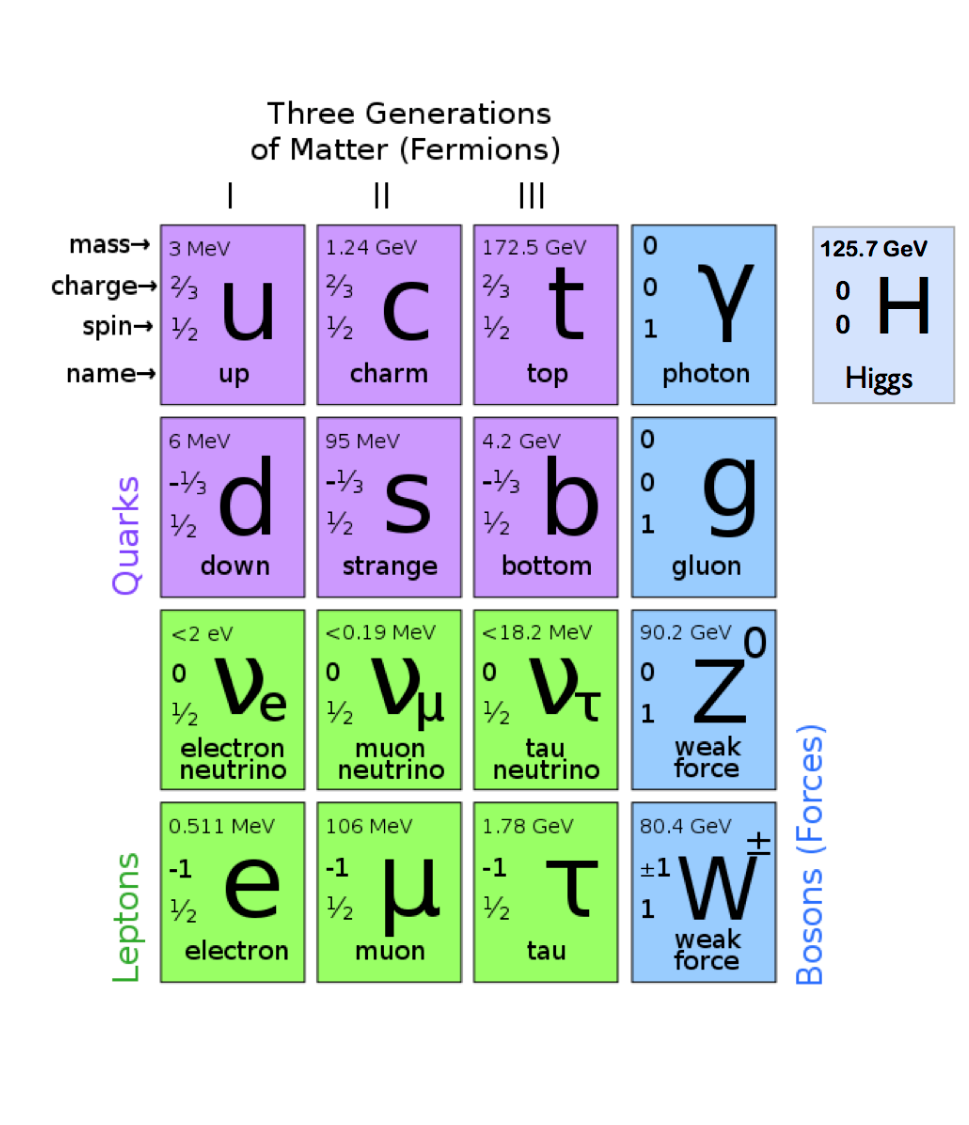
\includegraphics[width=0.7\textwidth]{figures/standard_model.pdf}
\caption[O Modelo Padrão de interação entre as partículas elementares]{
O Modelo Padrão de interação entre partículas elementares. Extraído de
\cite{tese_torres}.}
\label{fig:modelo_padrao}
\end{figure}

\subsection{Os bósons e as interações fundamentais}

As interações são comunicadas através dos bósons, partículas elementares
de campo das interações. Cada interação tem seu bóson característico: o gluôn (g); interação forte; 
o fóton $\gamma$; interação eletromagnética; e os bósons W e Z: interação fraca. Os bósons W e Z 
possuem respectivamente massa de aproximadamente 80 e 90~GeV. Esse fato limita o alcance da 
interação fraca a cerca de $10^{-3}$~fm, uma vez que uma partícula de massa $M$ só pode existir como 
parte de um estado intermediário por tempo $\hbar/Mc^2$, viajando uma distância não maior que
$\hbar/Mc$. O bóson W possui carga elétrica, enquanto o bóson Z é neutro, sendo sua própria 
antipartícula.

O bóson de Higgs (H), previsto inicialmente em 1964 pelo físico britânico Peter Higgs trabalhando
as ideias de Philip Anderson é descrita pelo mecanismo de Higgs sendo está a partícula que dá
massa a todas as outras, inclusive a ela mesma. Até então está partícula não tinha sido observada
devido as limitações tecnológicas da época. Outro problema referente à teoria era que esta não previa a faixa
de energia ou massa em que a partícula poderia ser observada. Porém em 4 de julho de 2012 essa observação
foi anunciada oficialmente em conjunto pelos grupos de físicos dos detectores \gls{atlas} e  \gls{cms}  do 
experimento \gls{lhc} em uma faixa de massa entre 125 e 127 $GeV$.

Por ser uma partícula instável o bóson de Higgs pode decair em $H\to 2Z$ e novamente
em $Z\to e^{+}e^{-}$, onde os elétrons são partículas estáveis e seu comportamento conhecido.
Existem outras formas de decaimento previstos pela teoria que não serão abordados neste
trabalho. Para realizar a observação de Higgs deve-se fazer o caminho inverso da reconstrução, ou seja,
detectar os dois pares de elétrons cujo a massa e outras propriedades físicas formam as
características do bóson Z. Por fim detectar o par intermediário de bósons que juntos reconstroem
as propriedades e massa do bóson H. Por ser o foco deste trabalho, o algoritmo de detecção
desses pares, chamado de   \gls{tap}, será abordado no capítulo seguinte.

Os físicos esperam adicionar a interação gravitacional através da partícula gráviton, que deverá 
ter rotação equivalente a 2 unidades de $\hbar$ e massa nula, entretanto não há nenhuma evidência 
experimental a favor ou contra sua existência \cite{Beiser}.

Os léptons podem ser subdivididos em dois grupos, um com massa e carga elétrica, idêntica e 
unitária: elétron, múon e táu; e outro neutro em carga e massa reduzida, estando relacionados 
com os léptons carregados: neutrino do elétron, neutrino do múon e neutrino do táon. Dos
léptons carregados, o múon e o táu só diferem dos elétrons na sua massa e no seu tempo de vida 
finitos, sendo o elétron o único estável.

Uma dificuldade da investigação experimental dos quarks é devido aos mesmos
nunca terem sido observados isoladamente.  Mesmo em colisões de altas energias os quarks 
se agrupam rapidamente em hádrons, formando jatos hadrônicos \cite{Intro_Nuclear}. Esse 
confinamento dos quarks ocorre porque a interação forte é similar a uma mola, quanto mais 
afastados, maior é a força de atração entre os quarks. Mas se energia suficiente for adicionada,
ao invés de um quark se liberar dos outros no hádron, a energia excedente produz um par de 
quark-antiquark \cite{Beiser}. Se dá ao nome dos sistemas compostos por quarks e gluôns de
hádrons, sendo os bárions e mésons os sistemas mais simples conhecidos. 

Um largo espectro dos bárions pode ser explicado como uma cápsula contendo
três quarks confinados por gluôns, sendo exemplos os prótons e nêutrons. Os mésons
são compostos essencialmente por um quark e antiquark ligados transitivamente por um gluôns. 
O próton é o único bárion estável\footnote{Teorias atuais
consideram que o próton decai com um tempo de vida muito longo, entretanto esse valor talvez seja 
maior que o valor mínimo detectado experimentalmente, de $10^{32}$~anos.  Para comparação, a 
idade do universo é de $10^{10}$~anos \cite{Beiser}.}, já o nêutron ($udd$), apesar de estável 
na estrutura atômica, quando isolado tem vida média de 15~minutos~\cite{Intro_Standard}. Finalmente, 
todos os mésons são instáveis e também são bósons, uma vez que mediam a interação
forte entre hádrons.

\section{O \emph{Large Hadron Collider} (LHC)}

O LHC começou a ser construído em 1998 com a colaboração de mais de 100 países, conta com um 
túnel de 27 km de circunferência, ao custo de aproximadamente  \euro $7,5 Bi$. Está em funcionando 
desde 10 de Setembro de 2008, tendo ocorrida sua primeira colisão entre prótons um ano e meio depois. Após as 
colisões entre 2010 e 2012, chamada de $run 1$, o \gls{lhc} passou por uma fase de $upgrade$
que perdurou até meados de 2015 quando foi finalmente religado. Para essa nova fase do calendário previsto
pela colaboração, chamado de $run 2$, espera-se colisões utilizando a energia nominal de 14TeV para
colisões de prótons.

\begin{figure}[h!t]
\centering
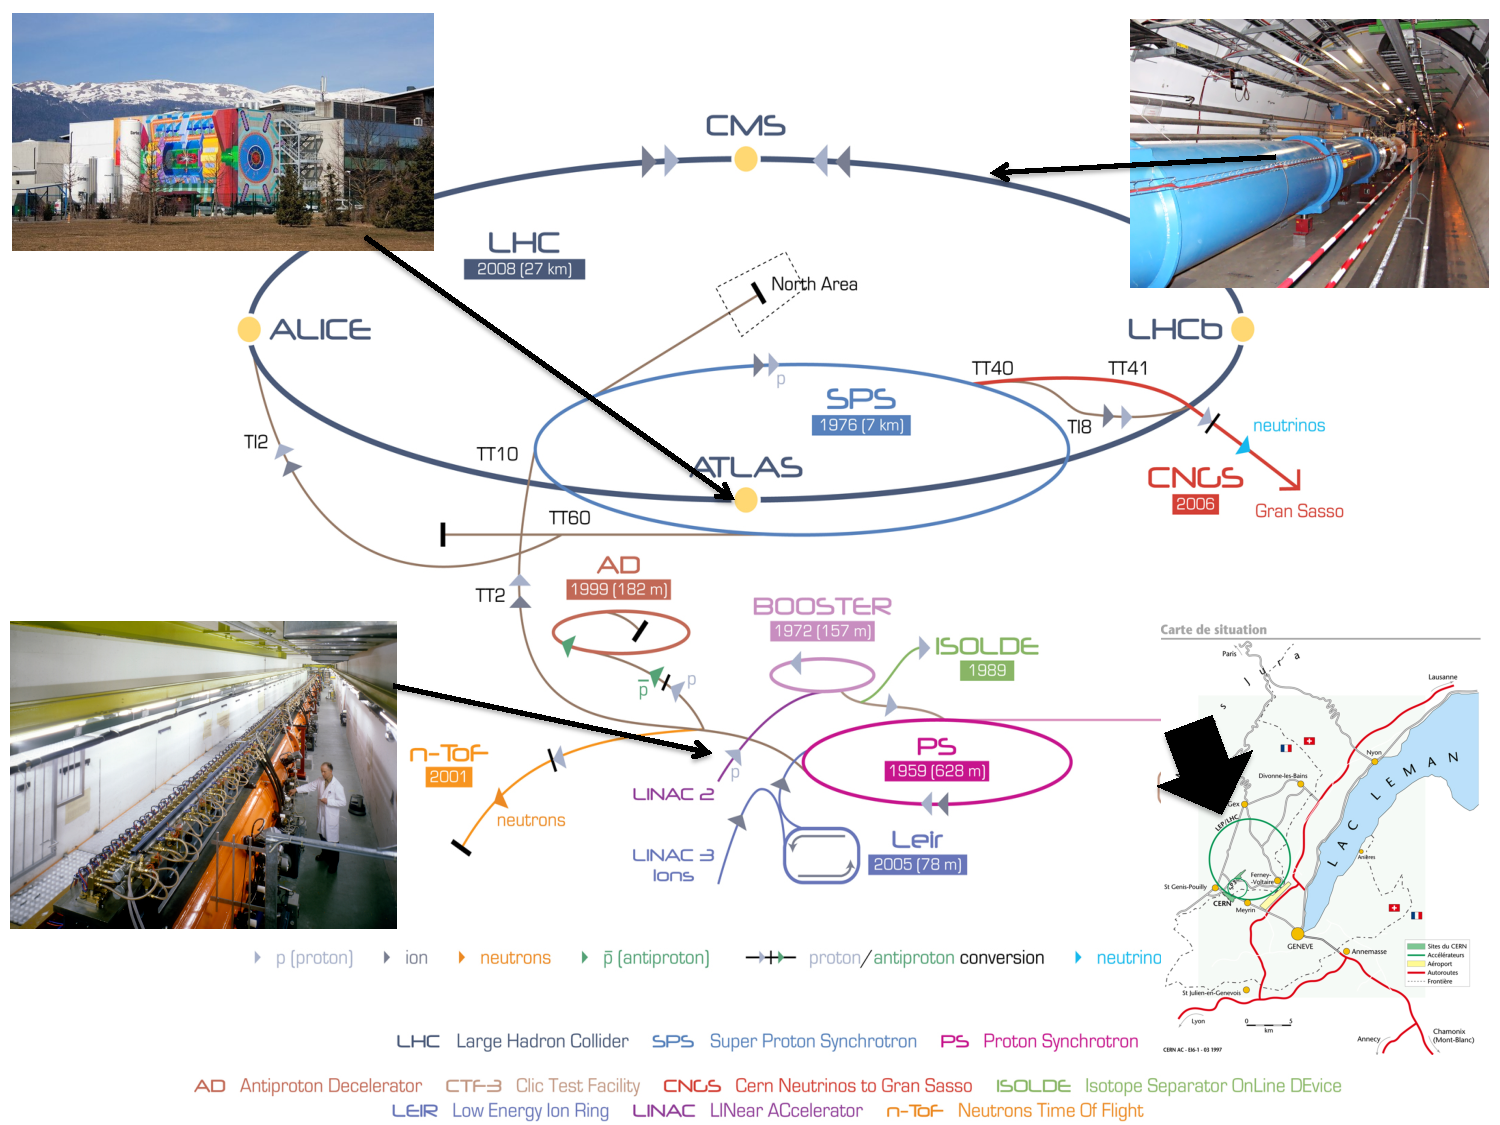
\includegraphics[width=\textwidth]{figures/lhc-overview.pdf}
\caption[A cadeia de aceleração do LHC]{
Os diferentes aceleradores da cadeia e detectores do CERN, extraído de
\cite{cern_accelerators}. A seta cinza claro corresponde ao sentido do
deslocamento de prótons nos aceleradores, No canto superior esquerdo
a foto do centro de controle do detector \gls{atlas}. No canto inferior esquerdo, a
foto do acelerador LINAC 2. No canto superior direito, a foto de uma seção do \gls{lhc}.
No canto inferior direito o mapa que mostra a localização do  \gls{lhc} na fronteira entre
a França e a Suíça.}
\label{fig:esquema_aceleradores}
\end{figure}

Para desenvolver a altíssima energia necessária para o experimento, o \gls{cern}
utiliza outros aceleradores construídos anteriormente, acelerando sequencialmente os pacotes 
de prótons até atenderem a energia desejada para a colisão. Na Figura \ref{fig:esquema_aceleradores} 
pode-se observar o esquema de aceleração, tanto para prótons, quanto para íons de chumbo. 
No caso dos prótons, o ciclo inicia-se na extração de prótons de átomos de hidrogênio que são
acelerados no \acrshort{linac} 2, um acelerador linear, que inicia a sequencia de aceleração, 
proporcionando-lhes uma energia de até 50 MeV.  Em seguida são utilizados síncrotrons, aceleradores 
circulares no qual as partículas seguem trajetórias circulares dirigidas por magnetos: \acrshort{booster} (1,4~GeV), 
\acrshort{psync} (25~GeV), \acrshort{sps} (450~GeV), até finalmente abastecer o \gls{lhc} com os pacotes 
de prótons. O \gls{lhc} também é um síncrotron, assim como grande parte dos aceleradores de altas 
energias anteriormente construídos \cite{lecture_slides_1,lecture_slides_2}.

Uma vez atingida a energia desejada para as colisões dos hádrons no \gls{lhc}, os pacotes serão então 
colididos nos \glspl{ip} experimentais. Esses pontos de colisão são formados pelos quatro principais detectores específicos 
para cada experimento. Os detectores \gls{atlas} e o \gls{cms} são utilizados para o estudo geral da matéria, o \gls{alice} 
é especializado em descobrir o mistério da matéria quente e densa que é brevemente criada quando da colisão de ions 
pesados a altas energias. Por fim, o \gls{lhcb} é um experimento desenvolvido para medidas precisas da violação da simetria 
e decaimentos raros de mésons com o quark b ou anti-b. A Figura ~\ref{fig:detectores} mostra uma visão global da 
arquitetura de cada um dos quatro principais detectores instalados no complexo. 

\begin{figure}[h!t]
\centering
\includegraphics[width=1\textwidth]{figures/detectors.pdf}
\caption[Os detectores do LHC.]{
Os quatro principais detectores instalados no complexo do \gls{lhc}. No canto superior esquerdo, o detector 
 \gls{atlas}. No canto superior direito, o detector \gls{alice}. No inferior direito, o \gls{lhcb} e, finalmente, no
 canto inferior esquerdo, o detector \gls{cms}.}
\label{fig:detectores}
\end{figure}

\newpage

\section{A Cinemática das Colisões}
\label{sssec:cinematica}

Ainda que não seja o objetivo do trabalho, um breve resumo da cinemática
relativística envolvida nas interações de partículas ajudará a entender algumas
das variáveis comumente utilizadas. 
Como o trabalho está englobado no experimento \gls{atlas}, irá se considerar o 
eixo de coordenadas adotado para o \gls{ip}1, ponto de inserção do mesmo. 

Normalmente se utilizam coordenadas esféricas ($p,\theta,\phi$), uma vez que 
essa é a geometria das colisões.
Seus eixos definidos em coordenadas retangulares estão dispostos 
na Figura~\ref{fig:atlas_p1_coord}, sendo o eixo \emph{z} a direção do feixe com
o lado positivo na direção do \gls{ip}8, o eixo
\emph{x} aponta na direção do centro do anel do \gls{lhc} e o eixo \emph{y}
aponta para a superfície.  
As transformações para coordenadas cilíndricas
são bem conhecidas e realizadas através da equação \ref{eq:transf_cil}.  
A física é simétrica em relação ao \gls{phi}, 
mas há correlação entre o
tipo de colisão com o \gls{theta}, onde geralmente quanto mais intensa a
interação ocorrida durante a colisão mais próximo de $90^\circ$ será esse
ângulo. O plano transverso é definido 
pelo corte transversal à direção de propagação do feixe, sendo o plano-xy do
sistema de coordenadas descrito, e a componente restante, paralela a direção de
propagação do feixe ($z$), é chamada de componente longitudinal.

\begin{figure}[h!t]
\centering
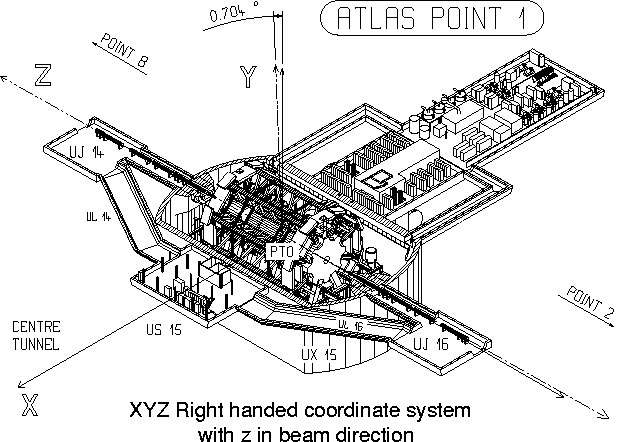
\includegraphics[width=0.7\textwidth]{figures/atlas_p1_coord.png}
\caption[O Sistema de Coordenadas adotado para o ATLAS]{O Sistema de Coordenadas adotado para o IP1, ponto de inserção do
experimento ATLAS. Extraído de \cite{tese_torres}.}
\label{fig:atlas_p1_coord}
\end{figure}

\begin{subequations}\label{eq:transf_cil}
\begin{equation}\label{eq:transf_phi}
\phi = arctan\left( \frac{x}{y} \right) \\
\end{equation}
\begin{equation}\label{eq:transf_theta}
\theta = arctan\left( \frac{x}{z} \right) 
\end{equation}
\end{subequations}

Estando interessado no momento das partículas
produzidas, a fim de se evitar as transformações de Lorentz, se faz mão de dois
parâmetros. Um deles, a \gls{y}, foi introduzido pela métrica de Minkowski
\cite{schlippe} e está definido na equação~\ref{eq:rapidez}.
O outro é o \gls{pt}, a projeção do momento no plano
transverso, dado pela Equação ~\ref{eq:pt}. 
Esses parâmetros são invariantes as transformações relativísticas 
longitudinais. O \gls{pl}, que não é conservado nas colisões entre hádrons por
esses não serem partículas ponto, pode ser obtido através
da Equação~\ref{eq:pl}. Outras duas variáveis que também
são projetadas no plano transverso são a \gls{mt} e \gls{Et}, obtidas através das
relações~\ref{eq:mt} e \ref{eq:Et}. Uma relação muito importante é a relação
massa-momento, dada pela equação~\ref{eq:rel_mom}.

\begin{equation}\label{eq:rapidez}
y = \frac{1}{2}ln\left(\frac{E+p_z}{E-p_z}\right)
\end{equation}

\begin{equation}\label{eq:rel_mom}
m^2c^4 = E^2 - p^2c^2
\end{equation}

\begin{subequations}\label{eq:proj_transv}
\begin{equation}\label{eq:pt}
p_T = p sen ( \theta ) = \sqrt{(p_x^2 + p_y^2)}
\end{equation}
\begin{equation}\label{eq:mt}
m_T = m^2 + p_T
\end{equation}
\begin{equation}\label{eq:Et}
E_T = E sen ( \theta )
\end{equation}
\end{subequations}

\begin{equation}\label{eq:pl}
p_L = p_z = m_T senh ( y )
\end{equation}

Os detectores absorvem a energia total (E) de grande parte das partículas
geradas nas colisões através de seus calorímetros, 
estando a mesma relacionada com a \gls{mt} por \ref{eq:etot}. Entretanto, na física de 
altas energias algumas aproximações podem
ser feitas de modo a facilitar a manipulação dos parâmetros. No caso ultrarrelativístico (quando $p \gg
m$) a rapidez se aproxima da \gls{eta}, parâmetro relacionado a \gls{theta}
através das equações \ref{eq:eta} \cite{pdg_book}.
Ainda, nesses casos a \gls{mt} tende a se aproximar de
\gls{pt}, e a energia total das partículas é predominantemente dado
pelo momento das partículas. Dessa forma, ao se projetar a energia absorvida
pelo calorímetro no plano transverso obtêm-se diretamente o \gls{pt} das
partículas, Equação~\ref{eq:e_pt}, obtida aplicando as relações \ref{eq:eta} em \ref{eq:etot}.

\begin{equation}\label{eq:etot}
E = m_{T}cosh(y) \approx m_{T}cosh(\eta) \approx p_{T}cosh(\eta)
\end{equation}
\begin{equation}\label{eq:eta}
\eta = -ln \left( tan\left( \frac{\theta}{2} \right) \right) \;,\; senh(\eta) =
cot(\theta) \;,\;  cosh(\eta) = 1 / sen(\theta) \;,\; tanh(\eta) = cos(\theta) 
\end{equation}
\begin{equation}\label{eq:e_pt}
p_T \approx \frac{E}{sen(\theta)}
\end{equation}



\section{O Detector de Partículas ATLAS}

\glsreset{atlas}
O ATLAS \cite{ATLAS_TDR,ATLAS_TDR2,paper_atlas}, Figura~\ref{fig:det_atlas}, é o maior 
dos detectores que operam no \gls{lhc}, medindo 45~metros de comprimento e 25~metros de altura 
e largura. Ele é um detector de propósito geral, registrando dados sobre os eventos de colisões de 
partículas que podem ser usados para estudos em diversas áreas da física. Cada uma de suas partes 
teve seus componentes construídos por um grupo diferente pertencente às instituições colaboradoras. 
Sua colaboração internacional envolve cerca de 2500 físicos de mais de 174 instituições 
e laboratórios de 38 países \cite{webATLAS}. Esses números incluem a \acrshort{ufrj}, que participa 
através da \acrshort{coppe}, da Escola Politécnica e do Instituto de Física. 

\begin{figure}[h!t]
\centering
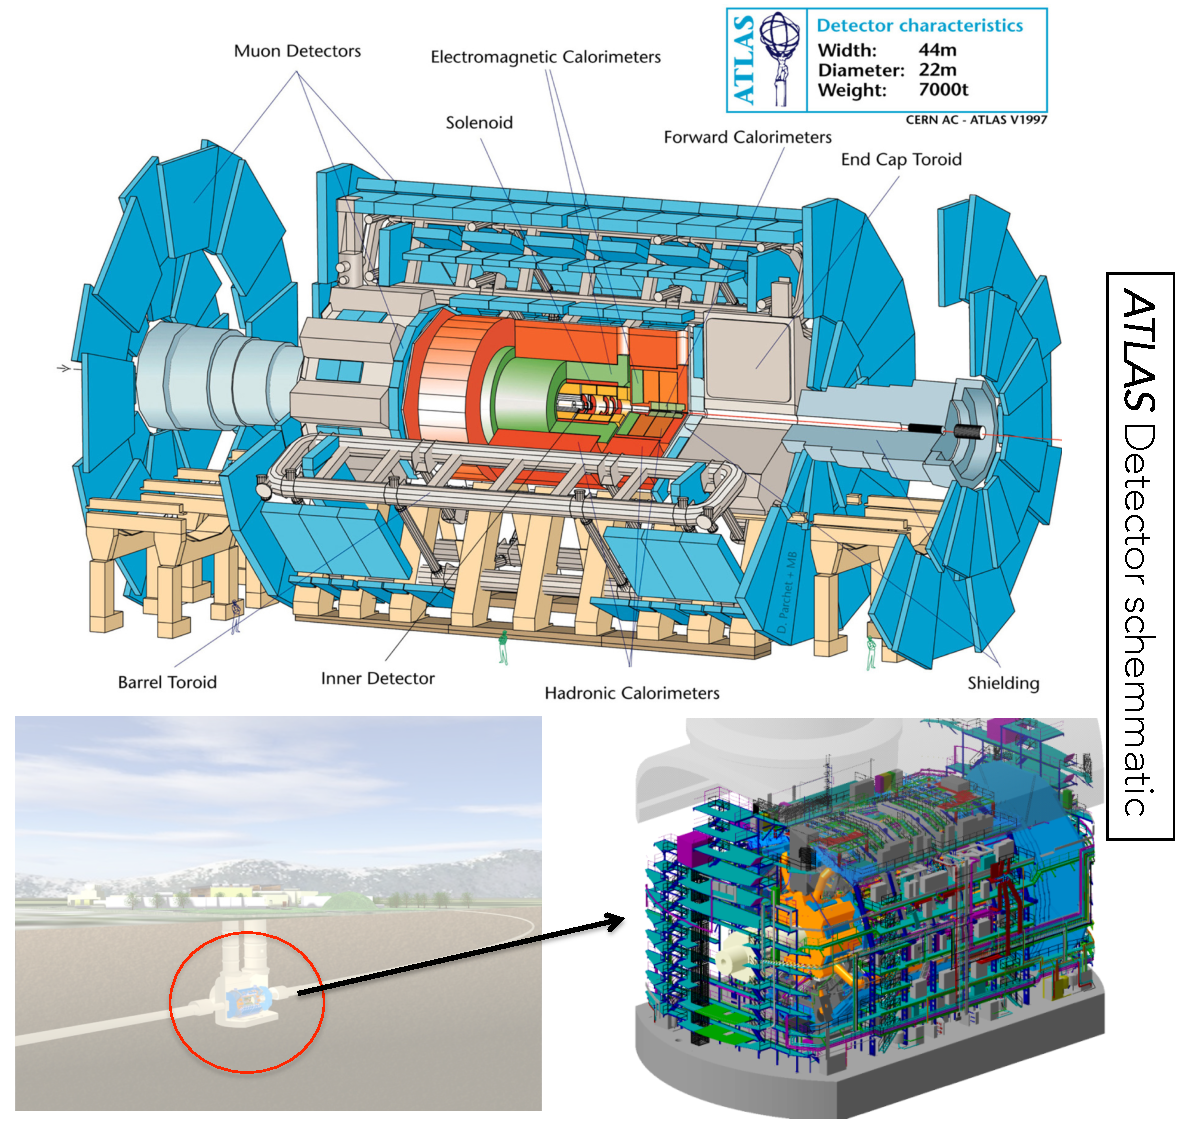
\includegraphics[width=1.1\textwidth]{figures/atlas-detector-overview.pdf}
\caption[O detector ATLAS.]{
O detector \gls{atlas} em diferentes níveis de detalhe. A ilustação do canto inferior esquerdo representa
a visão subterrânea da caverna onde está instalado o detector. O esquemático no canto direito representa
em detalhes a estrutura em volta do detector. A ilustração superior representa uma visão do detector em
cortes. Desde a parte mais interna, começando com o \gls{id}, até a camada mais externa dos subdetectores
de múons instalados em volta dos calorímetros.}
\label{fig:det_atlas}
\end{figure}


O \gls{atlas} possui 4 subdetectores, com um total de $~140$~M de canais de
leitura, sendo do mais interno para o mais externo:  \gls{id}\footnote{O \gls{id} 
também é referido como Detector de Traços.}, \gls{ecal}, \gls{hcal} e Espectrômetro 
de Múons. De maneira resumida, o \gls{id} identifica a trajetória e o momento de 
partículas carregadas, os calorímetros fazem a absorção das partículas medindo 
assim sua energia total, e o Espectrômetro de Múons é responsável exclusivamente 
pela detecção de múons. Através das assinaturas feitas pelas partículas nesses 
subdetectores é possível realizar a identificação das mesmas. A Figura~\ref{fig:particulas_atlas} 
contém um esboço de como as diferentes partículas idealmente interagem com os 
subdetectores do \gls{atlas}. 

Nas próximas subseções serão descritos em detalhes cada um dos sistemas instalados no detector, em especial 
o calorímetro eletromagnético e hadrônico responsáveis por absorver elétrons, fótons e partículas hadrônicas,
sendo estas as principais partículas a serem discriminadas pelo sistema proposto por este trabalho.

\begin{figure}[h!t]
\centering
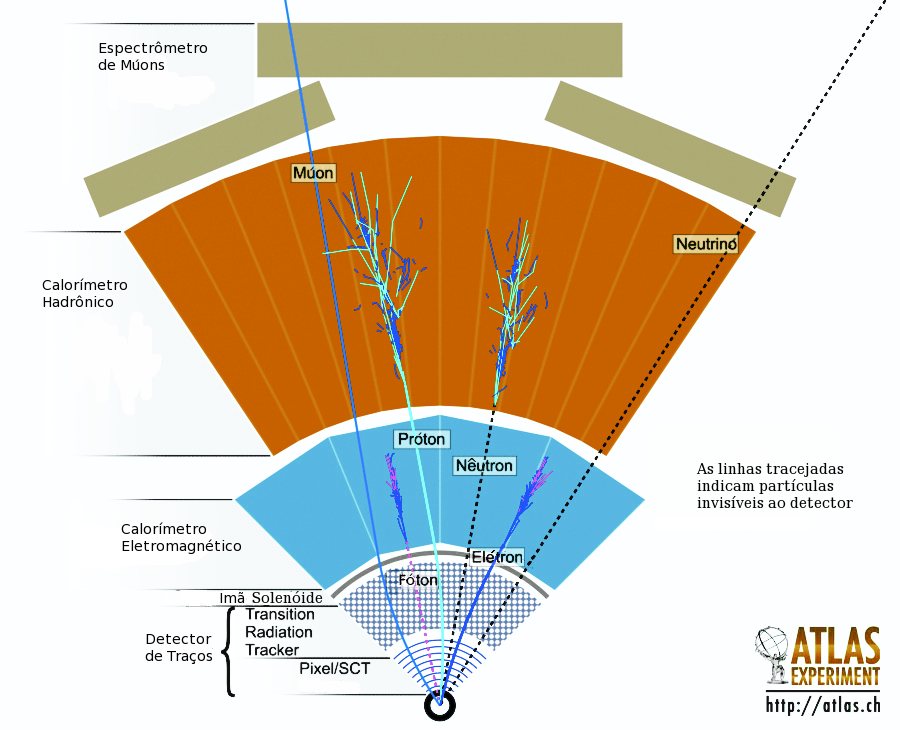
\includegraphics[width=0.8\textwidth]{figures/particulas_subdetectores_3.png}
\caption[Esboço contendo exemplos de interação de partículas com os
subdetectores do ATLAS]
{Um esboço contendo exemplos de interação de partículas com os
subdetectores do ATLAS. 
Apenas partículas carregadas eletricamente deixam traços no Detector Interno. 
Elétrons, pósitrons e fótons serão totalmente absorvidos pelo Calorímetro 
Eletromagnético. Ao Calorímetro Hadrônico, cabe a tarefa de absorver 
partículas com componentes hadrônicas, como nêutrons, prótons e outros mésons. Múons
mesmo contendo componentes eletromagnéticas devem atravessar os calorímetros com
facilidade, sendo somente detectados pelo Espectrômetro de Múons. Léptons Neutrinos não
são detectados por nenhum dos subdetectores do ATLAS. Adaptado de \cite{particulas_atlas}.}
\label{fig:particulas_atlas}
\end{figure}

\newpage

\glsreset{id}

\subsection{O Detector Interno}
\label{ssec:det_int}

O \gls{id} \cite{inner_tdr1,inner_tdr2}, Figura~\ref{fig:det_interno}, é o responsável pela identificação das 
trajetórias de partículas carregadas, medir o seu momento, o
vértice primário\footnote{local aonde ocorreu a colisão dos hádrons no detector}, os
vértices de decaimentos de partículas e a distância entre o vértice primário e o ponto mais próximo do traço
\cite{tese_jatos,ATLAS_TDR}. Ele cobre uma região com completa cobertura em
\gls{phi} de maneira simétrica para $|\gls{eta}| < 2,5$, a chamada região de precisão
do detector.  


A medição do momento é realizada através da deflação das partículas pelo
\gls{campmag} e sua resolução depende da \gls{respos}, da magnitude de
\gls{campmag} e do \gls{comprimento} do rastreador de acordo com a Equação \ref{eq:res_mom}
\cite{lecture_slides_1,lecture_slides_2}. O \gls{campmag} é fornecido pelo
\gls{cs} restando apenas dois parâmetros a serem explorados, o \gls{respos} e \gls{comprimento}. 
A resolução de vértices é proporcional a capacidade de reconstrução da trajetória da partícula e 
assim como o momento é inversamente proporcional à posição \gls{respos}. 

Também é necessário uma baixa granularidade, devido há uma grande densidade de
traços gerados no \gls{lhc} resultando em $\approx$10.000 traços no intervalo de 
100~$n$s~\cite{resumo_ATLAS}, e à baixa quantidades de material no \gls{id} 
para que seja possível realizar medições nos calorímetros sem que as partículas 
interajam e percam energia nos componentes deste detector.

\begin{equation}\label{eq:res_mom}
\frac{\delta p_T}{p_T} = \frac{p_T \sigma_p}{0,3Bl^2} [GeV,T,m]
\end{equation}

\begin{figure}[h!t]
    \label{fig:det_interno}
    \begin{center}
        \subfigure[Seção de corte do Detector Interno mostrando seus subsistemas. Extraído de
\cite{paper_atlas}.  ]{%
            \label{fig:id_secao}
            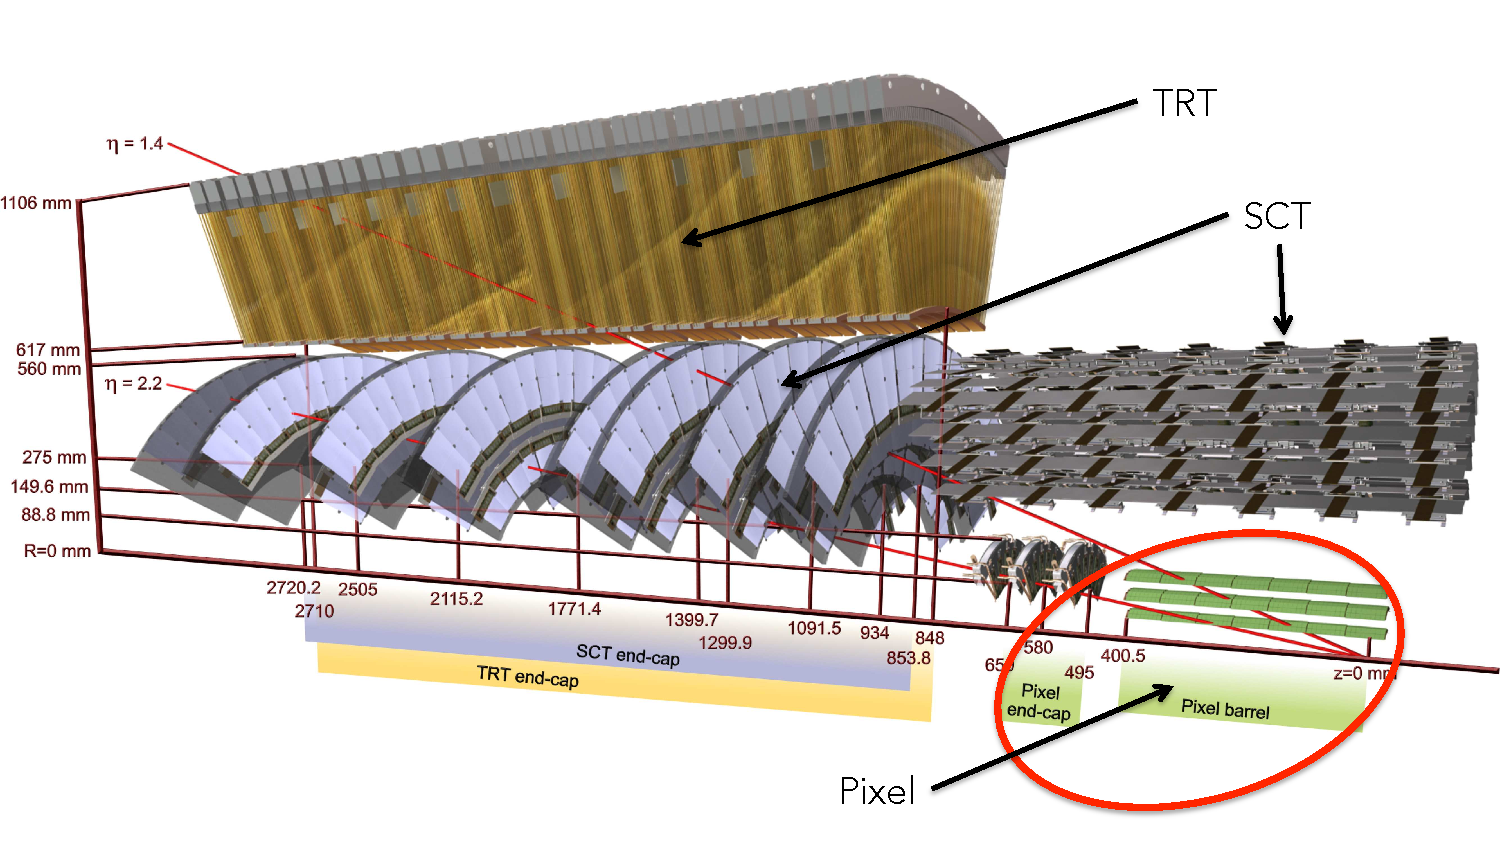
\includegraphics[width=\textwidth]{figures/id_lateral_2.pdf}
        }\\
        \subfigure[Esboço do Detector Interno, contendo suas dimensões e
pseudorrapidez relacionas. Extraído de \cite{paper_atlas}.]{%
            \label{fig:id_eta}
            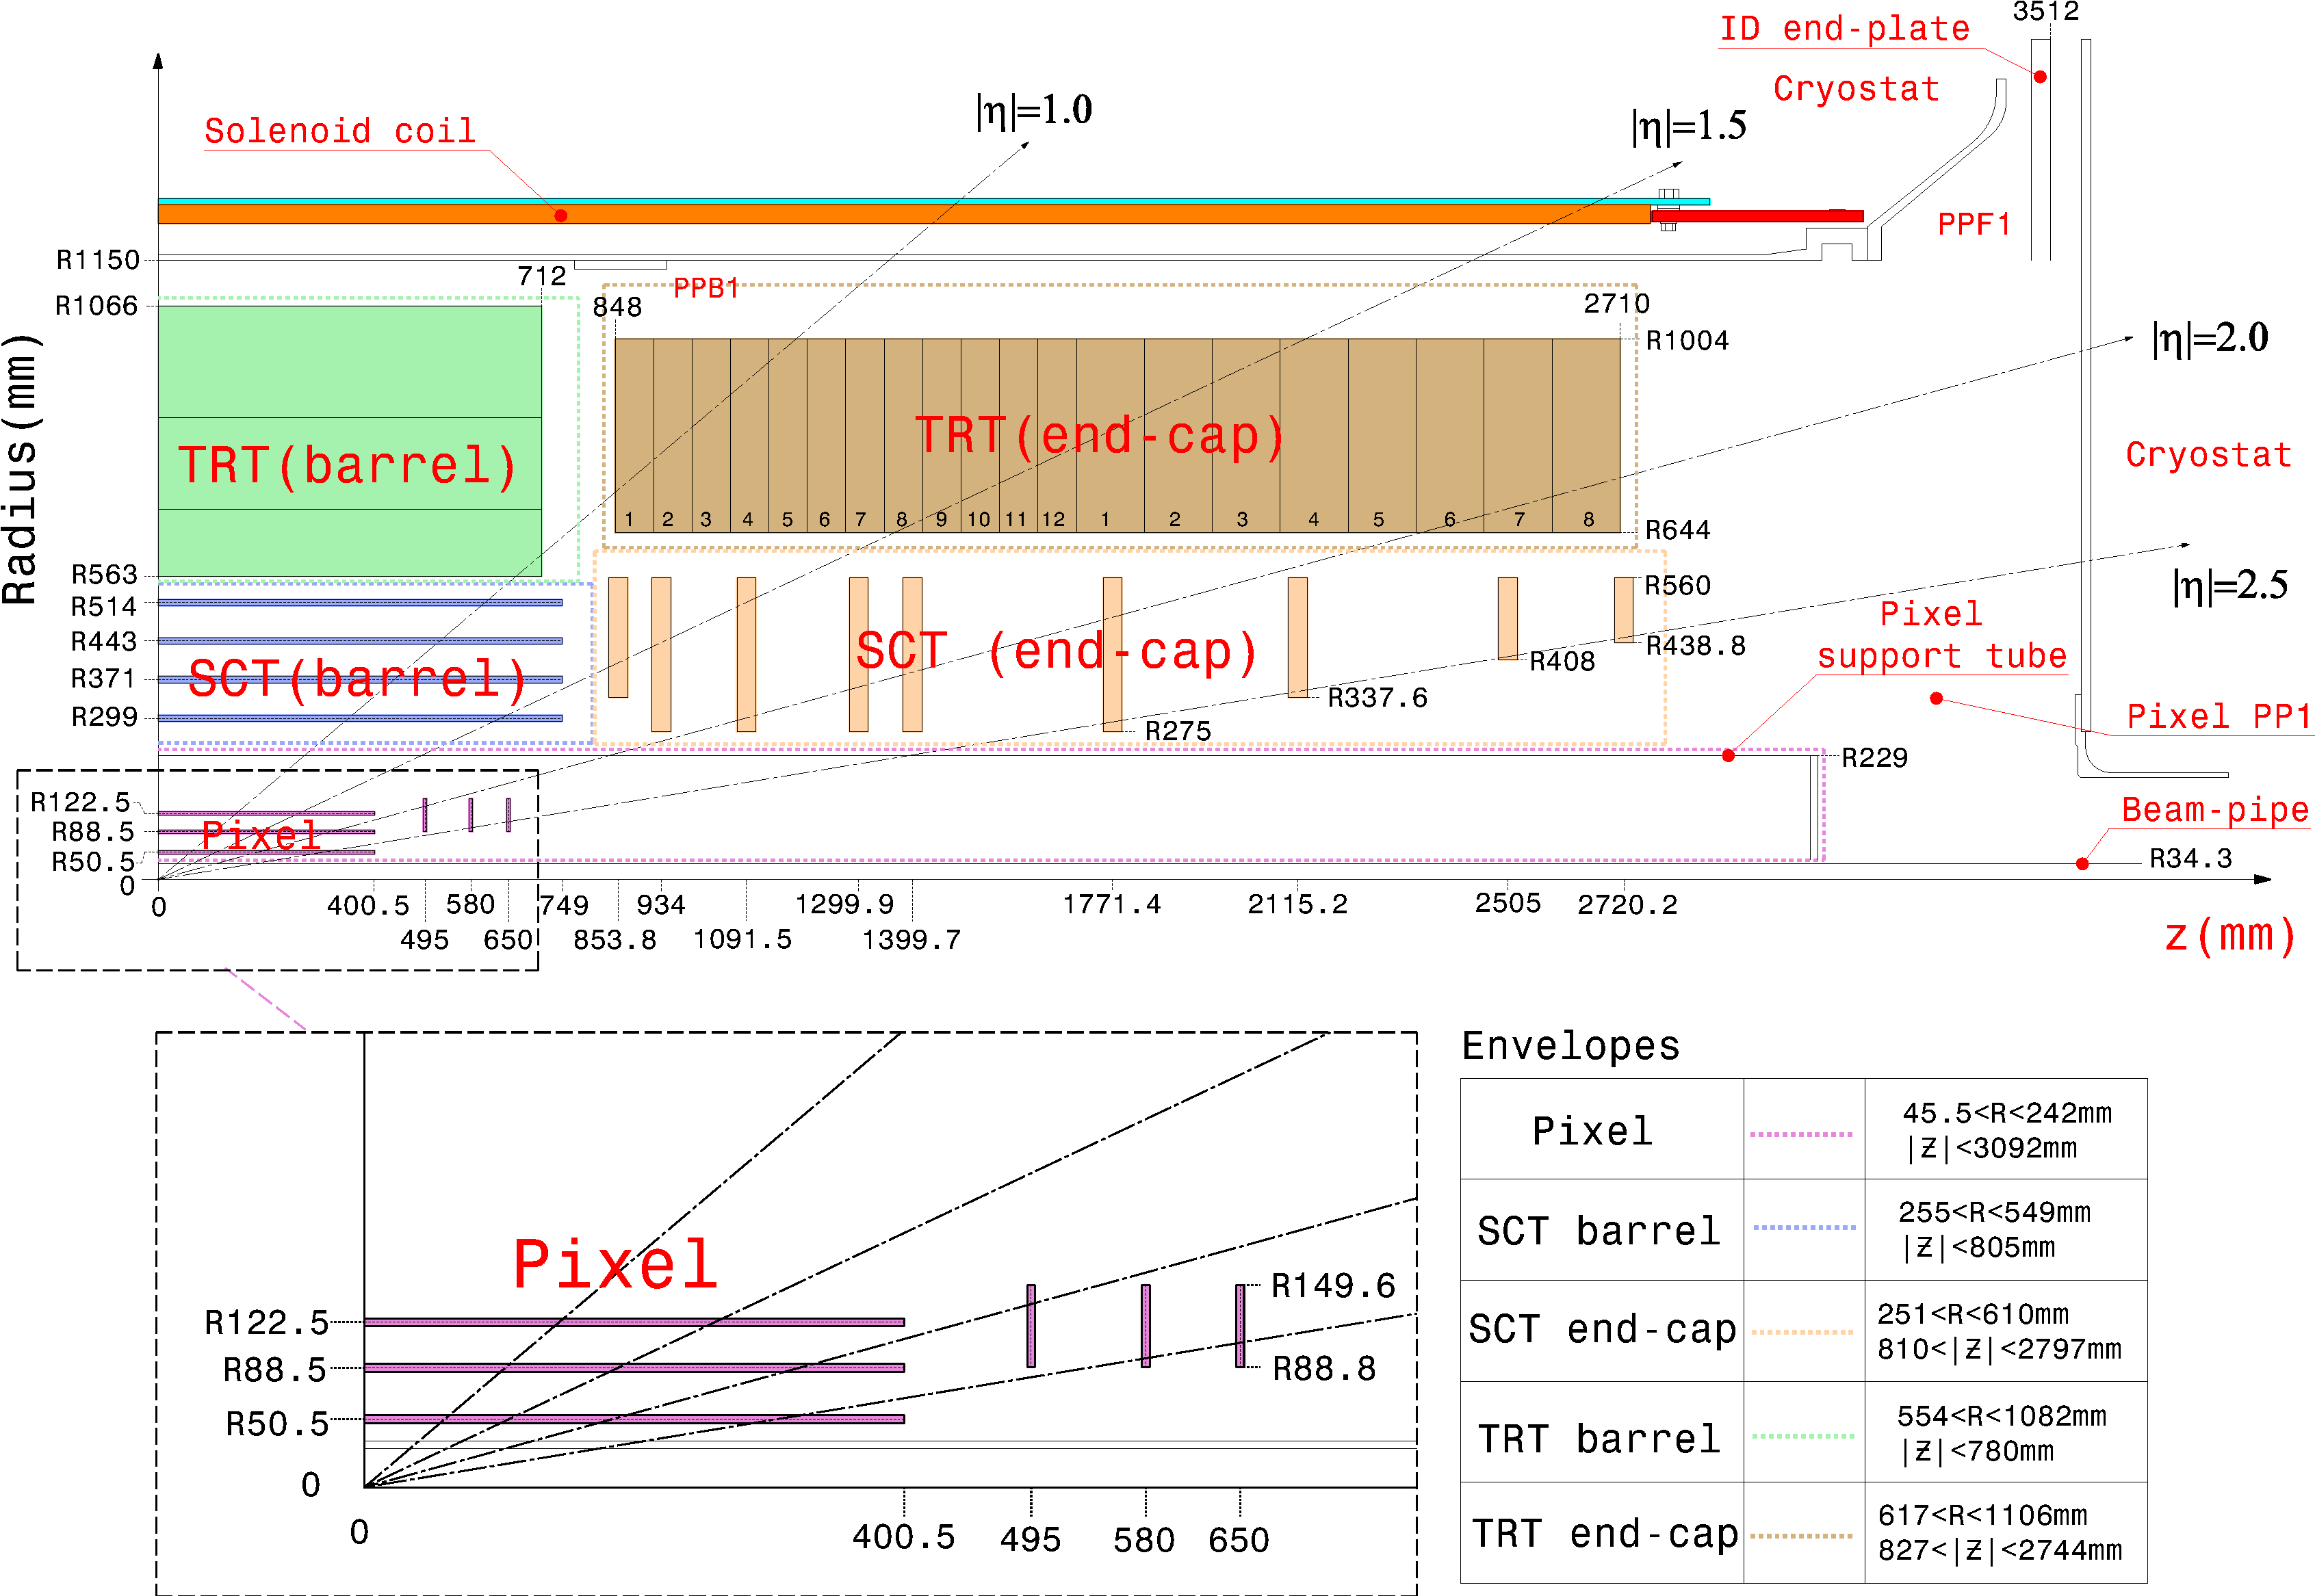
\includegraphics[width=.8\textwidth]{figures/id_eta.pdf}
        }
    \end{center}
    \caption[O Detector Interno (ID)]{O Detector Interno.}%
\end{figure}

O \gls{id} dispõe de dois medidores de alta precisão, que exploram a redução 
de \gls{respos} para melhorar a resolução do detector. Os detectores de alta 
precisão são formados pelos Detectores de Pixel e \gls{sct}. O \gls{trt}
explora o acréscimo do \gls{comprimento} do detector em busca de uma melhor
resolução de momento. Um resumo das capacidades de
cada um dos detectores é fornecido na Tabela~\ref{tab:info_id}.

\begin{table}
\centering
\resizebox{\textwidth}{!}{
\begin{tabular}{lp{5cm}cccp{2cm}}
\hline
\hline
\textbf{Sistema} & \textbf{Posição} & \textbf{Área} ($\text{m}^2$) & \textbf{\gls{respos}
($\mu$m)} & \textbf{Canais ($10^6$)} & \textbf{Cobertura em $|\eta|$} \\
\hline
\hline
Pixeis & 1 camada removível no barril (Camada B) & 0,2 & R$\phi$ = 12, z = 66 & 16
& $\leq 2,5$ \\
& 2 camadas no barril & 1,4 & R$\phi$ = 12, z = 66 & 81 
& $\leq 1,7$ \\
& 3 discos nas tampas de cada lado & 0,7 & R$\phi$ = 12, R = 77 & 43 
& $1,7-2,5$ \\
\hline
SCT & 4 camadas no barril & 34,4 & R$\phi$ = 16, z = 580 & 3,2
& $\leq 1,4$ \\
& 9 discos nas tampas de cada lado & 26,7 & R$\phi$ = 16, R = 580 & 3,0
& $1,4-2,5$ \\
\hline
TRT & Canudos axiais no barril &  & 170 (por canudo) & 0,1
& $\leq 0,7$ \\
& Canudos radiais nas tampas &  & 170 (por canudo) & 0,32
& $0,7-2,5$\\
\hline
\hline
\end{tabular}
}
\caption[Parâmetros do ID]
{Parâmetros do ID. As resoluções estão citadas em valores típicos (a
resolução verdadeira em cada detector depende do ângulo de impacto). Adaptado de
\cite{ATLAS_TDR}.}
\label{tab:info_id}
\end{table}



\subsubsection{Detector de Pixeis}
\label{sssec:pixeis}

A maior granularidade é atingida pelos pixels semicondutores próximos
ao vértice da colisão, entretanto o número de camadas de precisão devem ser
limitadas devido à grande quantidade de material introduzida e ao seu alto
custo. Dessa forma, o Detector de Pixel utilizado foi projetado para
fornecer apenas três pontos de alta precisão. Ele determina a resolução do
\gls{d0} e a habilidade do \gls{id} de encontrar partículas de curta
vida como hádrons B e táons. Um total de 140~M de canais de
leitura estão dispostos com um afastamento de 50~$\mu$m na direção R$\phi$, 
mesma direção que o plano transverso, e 300 $\mu$m em z. 
O sistema consiste de três barris a uma distância radial
média de $\sim$5~cm, 10~cm, 13~cm, e três tampas em cada lado entre uma distância 
radial de 11 e 20~cm.

\subsubsection{Detector de Rastreamento por Semicondutores (SCT)}
\label{sssec:sct}

O \gls{sct} foi projetado para fornecer oito pontos de precisão por traço na
região intermediária do \gls{id}, contribuindo tanto para a medição do momento,
parâmetro de impacto e posição do vértice primário, quanto provendo bom
reconhecimento de padrões pelo uso de alta granularidade. O seu barril usa oito
camadas de microfibras de silicone para gerar precisão nos pontos nas
coordenadas de R$\phi$ e z. Cada componente mede $6,36\times6,40 \text{cm}^2$ com 768 canais de
leitura com 80~$\mu$m de afastamento. A tampa possui construção similar, mas usa
tiras cilíndricas, formando um conjunto alinhado radialmente. Ela possui cerca de 61~$m^2$ 
de detectores de silicone, com 6,2~M de canais, que permitem distinguir
dois traços separados por cerca de $\sim200~\mu$m.

\subsubsection{Detector de Rastreamento por Transição de Radiação (TRT)}
\label{sssec:trt}

Por outro lado, o \gls{trt} explora a medição contínua do traço com uma
quantidade bem menor de material e custo. Ele fornece cerca de 36 pontos por
traço, melhorando assim a resolução do momento ao explorar um maior
\gls{comprimento}. Ele se baseia em detectores de canudos, que podem operar nas
grandes taxas esperadas no \gls{lhc} em virtude de seus pequenos diâmetros e
isolamento dos sensores dentro de volumes individuais de gás. A capacidade de
identificação de elétrons é adicionada aplicando xenônio para detectar fótons de
radiação transiente em seu radiador entre os canudos. O barril contém cerca de
50.000~canudos, divididos em dois no seu centro para reduzir a ocupação, e sua
leitura em cada ponta. A tampa contém~320.000 canudos radiais, com a leitura na
ponta externa. As medições realizadas pelos canais são em formas de
impulsos e dão uma resolução espacial de 170~$\mu$m por canudo.


%----------------------------- CALORIMETRIA --------------------------------
\newpage
\subsection{O Sistema de Calorimetria}
\label{ssec:calorimetria}

Na calorimetria \cite{wigmans,tese_torres}, a energia das partículas é 
absorvida através de suas interações com o calorímetro, sendo assim um processo 
de detecção destrutivo, ou seja, não é possível realizá-lo novamente. Os calorímetros 
podem ser de dois tipos: homogêneos ou de amostragem. 

O método de amostragem utiliza-se de dois materiais: o material passivo 
responsável pela interação com a partícula, realizando a absorção de energia da
partícula; e o ativo, no qual ocorre a geração, ou amostragem, do sinal. 
Calorímetros homogêneos utilizam um único material para realizar as duas
tarefas: a de interagir com a partícula e gerar sinal; e por isso apresentam melhor resolução de energia 
que os de amostragem, uma vez que parte da energia das partículas nas interações com o
material passivo dos calorímetros de amostragem é perdida. Por sua vez, calorímetros de amostragem são
mais baratos e por isso utilizados em sistemas de detecção muito grandes, como o
\gls{atlas}. Além disso, a resolução de energia do calorímetro para o método de 
amostragem melhora para partículas de maior energia.

Uma partícula, ao transpassar o material do calorímetro geralmente interage de
forma a excitar o meio ou aquecê-lo. O tipo de interação ocorrida depende da
quantidade de energia da partícula, de sua natureza, assim como do
meio, podendo ter como resultado interações eletromagnéticas, fortes, e mais 
raramente, fracas. Em altas energias os processos de interação com o meio 
criam uma cadeia contínua de eventos, provocando os chamados chuveiros de partículas. 


\subsubsection{Utilização dos calorímetros para identificação de partículas}
\label{par:cal_part_id}

\glsreset{ecal}
\glsreset{hcal}

Sabendo como as partículas hadrônicas e eletromagnéticas reagem com
o calorímetro, cabe fazer algumas considerações sobre os calorímetros
responsáveis pela detecção das mesmas. 

O \gls{ecal} é responsável pela absorção de partículas puramente \gls{em}, ou seja, que não têm componentes
\gls{had}, como os léptons carregados e fótons. Os múons, embora façam parte do
grupo de partículas puramente \gls{em}, atravessam
grandes quantidades de material perdendo pouca energia uma vez que são bem mais
maciços que elétrons e por isso é utilizado o Espectrômetro de Múons para
detectá-los. Táons são ainda mais maciços e precisariam de mais
material que os múons para serem detectados. Entretanto, eles tem tempo de vida muito curto e
decaem em múons (ou elétrons) e mais dois neutrinos antes de atingirem o detector, sendo detectados
indiretamente através dos resíduos de seu decaimento. Com isso, apenas elétrons,
pósitrons e fótons são detectados no \gls{ecal}, mas vale ter em mente que eles
podem ser estados finais de outras partículas. 

Por outro lado, o \gls{hcal} deve absorver todas as partículas \gls{had}, como os jatos
\gls{had} que podem ser resíduos de um \gls{ue} e \gls{mbias}, ou até mesmo de
um decaimento. Alguns canais de interesse desejam encontrar jatos, como 
o decaimento do bóson W em altos \gls{pt} para $|\gls{eta}|<3$: $W\rightarrow jato-jato$. 
Entretanto, é necessário separar esses jatos dos criados pelo ruído 
gerados por \gls{mbias} e \glspl{ue}, e para isso o \gls{hcal} deve ser capaz de
separar um jato de um decaimento duplo em jatos próximos, sendo
necessário uma granularidade maior nessa região.

Quanto maior o número atômico do meio, maior será a profundidade no qual um
chuveiro \gls{had} irá se propagar no mesmo, quando em comparação com um chuveiro
\gls{em} de mesma energia. Isso culmina na disposição
dos \gls{ecal} serem anteriores ao dos \gls{hcal}, uma vez que é inútil, assim, utilizar calorímetros com a 
configuração espacial oposta, já que todos os chuveiros de partículas se
extinguiriam no \gls{hcal}, não atingindo o \gls{ecal}. Ainda, é interessante a
utilização de materiais com grandes números atômicos no \gls{ecal} para
garantir, por esse motivo, a menor deposição de energia possível de partículas
\gls{had} no mesmo.

Ainda, o perfil de chuveiros \gls{had} é mais largo que o de chuveiros
\gls{em}. Essa ocorrência é muito explorada para realizar a discriminação 
entre as partículas que interagem com os calorímetros, buscando perfis de chuveiros
justos para partículas \gls{em}. Ela tem como consequência 
a menor granularidade no \gls{ecal} quando comparados com os \gls{hcal}, já que
para realizar a discriminação é necessário que o calorímetro tenha resolução
para discernir entre os chuveiros. Ao mesmo tempo, se faz desnecessário
utilizar altas granularidades no \gls{hcal}, justamente pelos chuveiros se
espalharem por uma região maior.


\subsubsection{Os subsistemas de calorimetria e suas topologias}
\label{sssec:cal_estrutura}

O Sistema de Calorimetria \cite{cal_tdr,ecal_tdr,hcal_tdr} do \gls{atlas}, retratado na
Figura~\ref{fig:cal_atlas}, consistem de calorímetros de amostragem com 
simetria e cobertura total em \gls{phi}.

\begin{figure}[h!t]
\centering
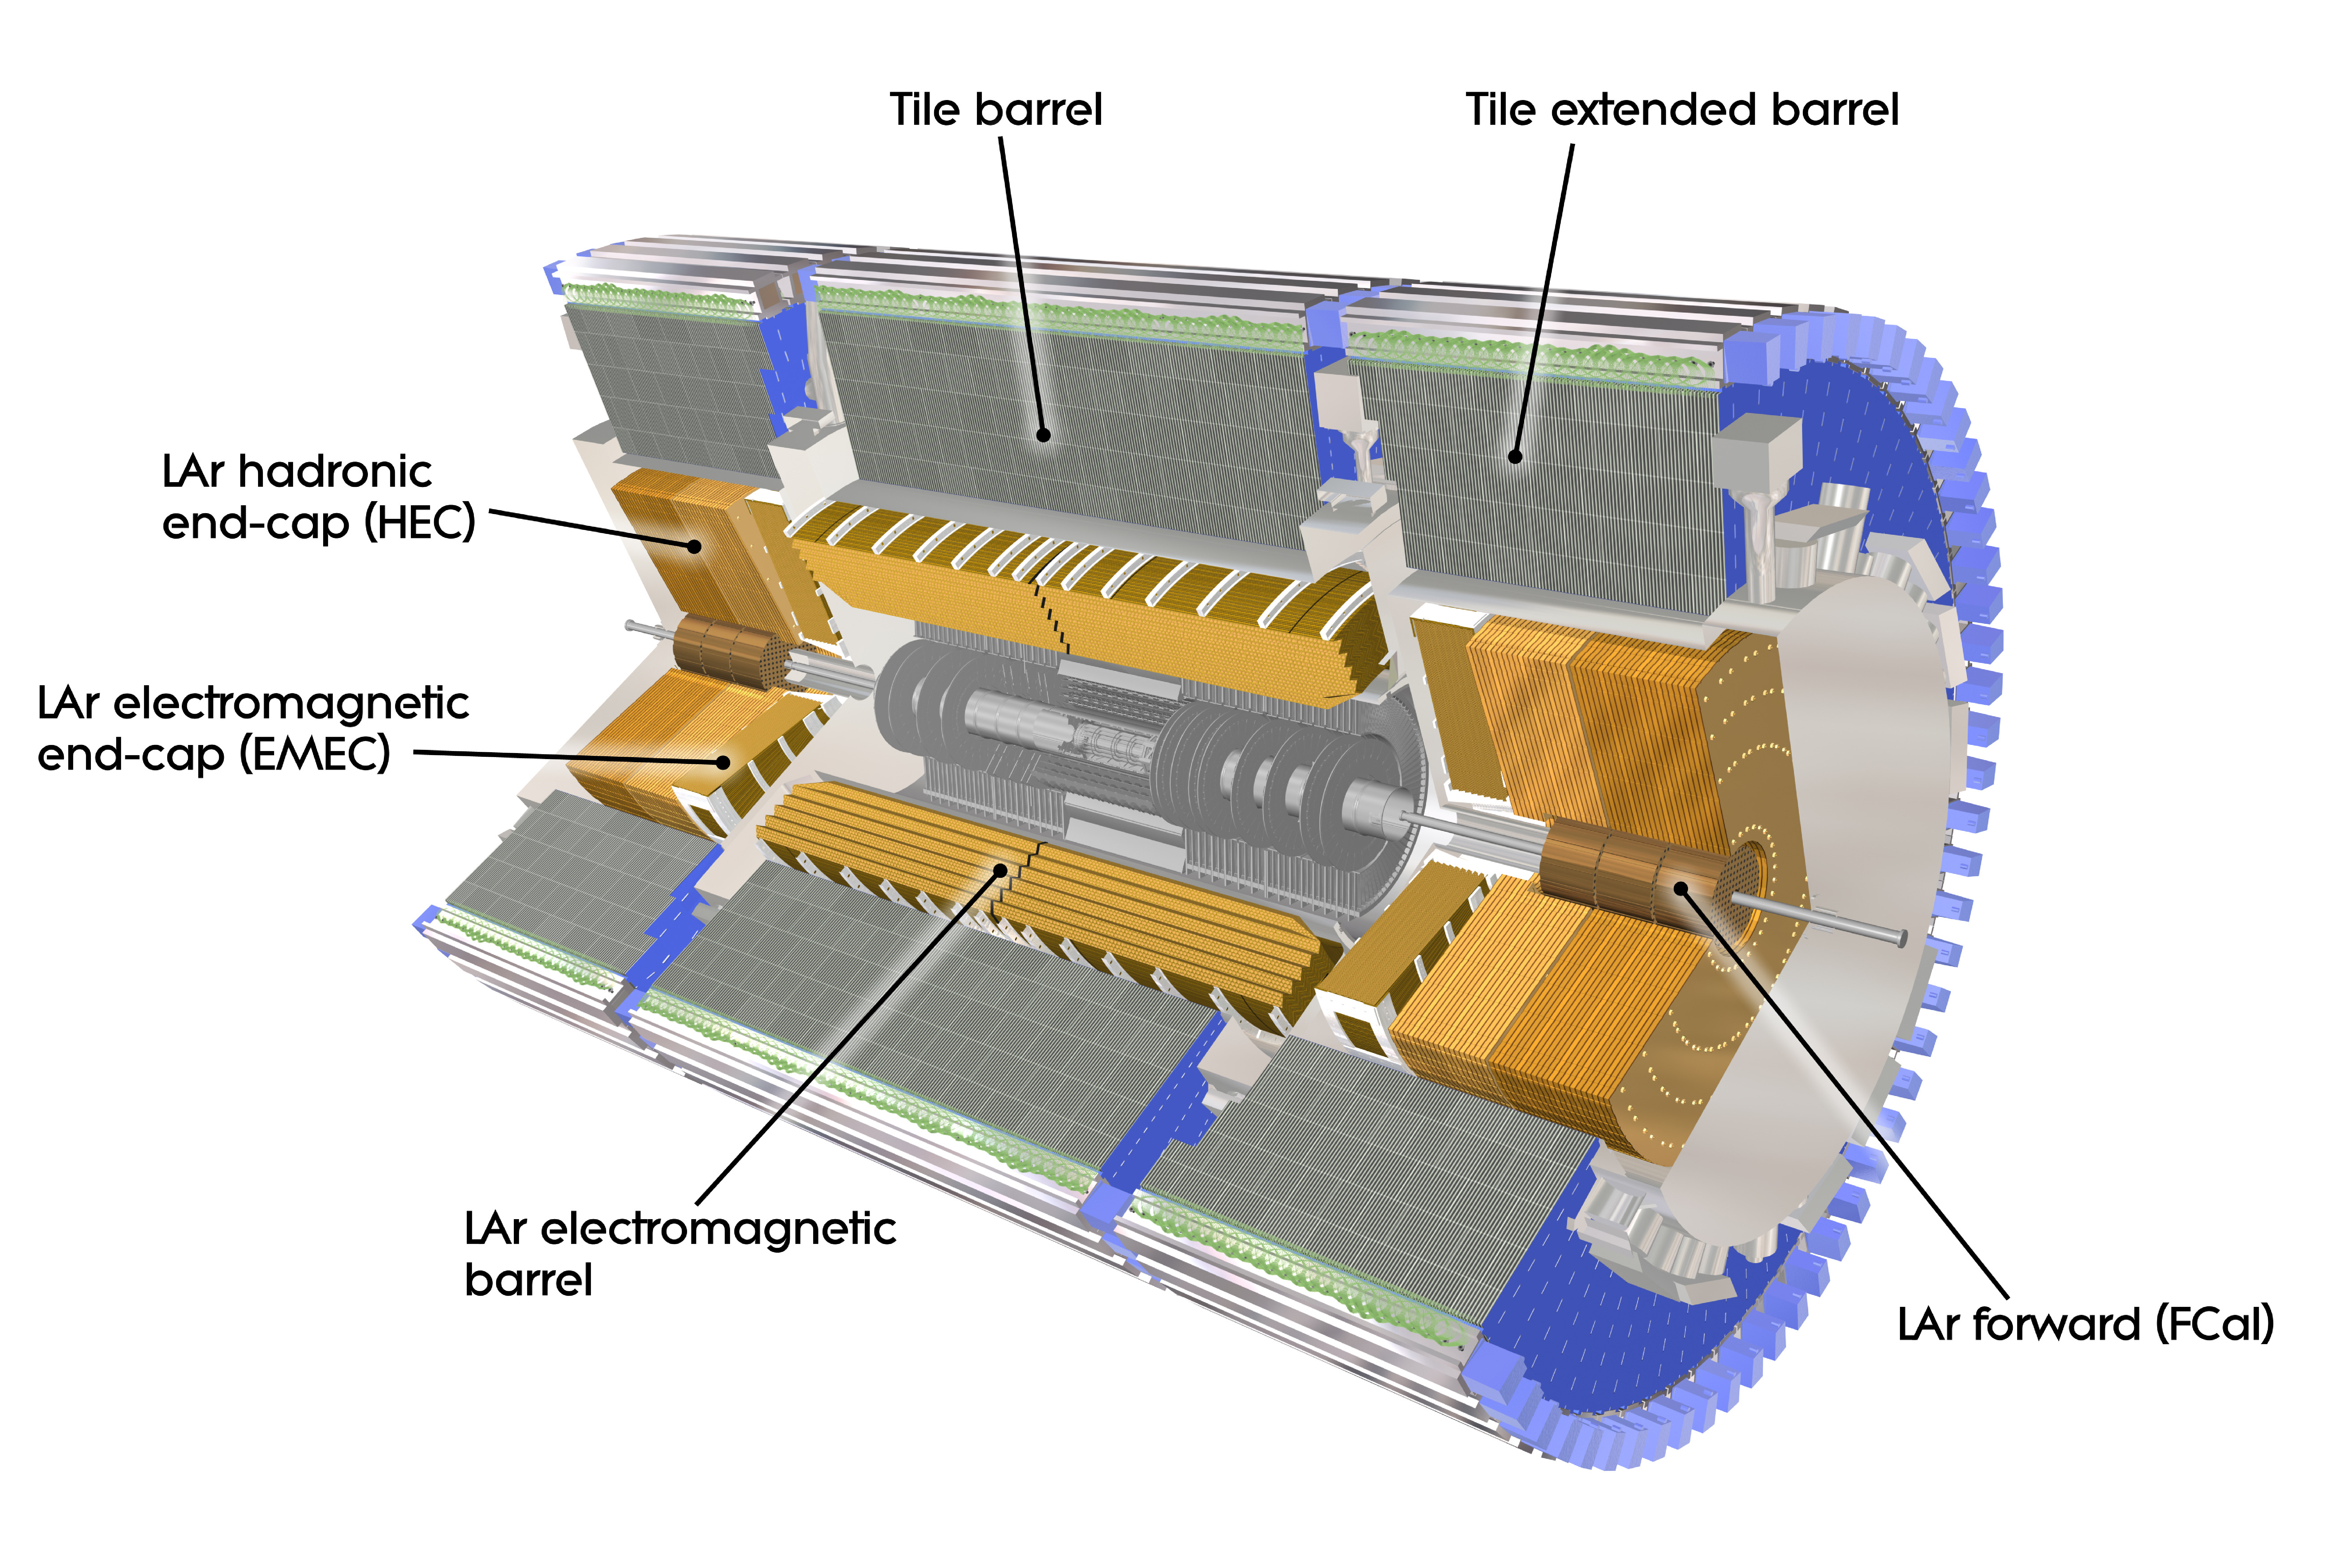
\includegraphics[width=\textwidth]{figures/calorimetros.pdf}
\caption[Os diversos subsistemas de calorimetria do ATLAS]{
Os diversos calorímetros do ATLAS. Extraído de
\cite{atlas_calorimeter_photo}.}
\label{fig:cal_atlas}
\end{figure}

O \gls{ecal} do \gls{atlas} jaz na parte mais interna do detector e cobre uma região de 
pseudorrapidez $|\gls{eta}|<3,2$. Ele pode ser dividido no
\gls{emb}, que cobre uma região pseudorrapidez de $|\gls{eta}|<1,475$, 
e por suas \glspl{emec}, cobrindo por sua vez a região de $1,375<|\gls{eta}|<3,2$.

Seu \gls{hcal} cobre a mesma região de pseudorrapidez que o \gls{ecal}, envolvendo
o mesmo. O seu barril alcança até $|\gls{eta}|<1,0$, sendo adicionado uma
extensão para aumentar o alcance na região de $0,8<|\gls{eta}|<1,7$. Juntos eles
compõem o \gls{tilecal}. Finalmente, as \glspl{hec} cobrem a região de $1,5<|\gls{eta}|<3,2$. 

Um calorímetro de menor precisão, \gls{fcal}, 
é utilizado para cobrir a região mais próxima do tubo do feixe, de
$3,1<|\gls{eta}|<4,9$, compondo uma extensão ao \gls{ecal} através de sua primeira camada,  
e ao \gls{hcal} com suas segunda e terceira camadas. 

Para todas as regiões de transição entre calorímetros citadas 
há a extensão dos mesmos de modo que haja sobreposição, 
com o objetivo de evitar a queda súbita de material \cite{paper_atlas}. 

A segmentação, granularidade e número de canais (um total de $\sim190.000$) 
em cada um dos calorímetros está contida
na Tabela \ref{tab:calo}. Uma observação interessante é a queda da granularidade
conforme o aumento de \gls{eta}. Esse fato se deve a região de precisão do 
\gls{atlas} estar limitada para $|\gls{eta}| < 2,5$, consequência da capacidade do
\gls{id} de suportar radiação\fnref{fn:radiacao}. A granularidade do
\gls{hcal} é menor que a do \gls{ecal}, devido a maior largura de chuveiros
\gls{had}. Nas regiões de maior $|\gls{eta}|$, principalmente no \gls{fcal}, 
a tarefa principal do calorímetro é reconstruir jatos e medir a
\gls{Etmiss}, de modo que uma granularidade mais grosseira é aceitável.
Ainda, é possível observar um decaimento da granularidade conforme o acréscimo
das camadas de segmentação longitudinais, o que ocorre devido a expansão da
espessura lateral do chuveiro conforme a propagação do mesmo pelo calorímetro.


\subsubsection{Barril (EMB) e Tampas (EMEC) do Calorímetro Eletromagnético}
\label{par:ecal_prec}

Os \glspl{ecal} de precisão, compostos pelo \gls{emb} e \glspl{emec}, 
utilizam detectores de \gls{lar}, contendo absorvedores compostos por eletrodos 
de cobre, o seu meio ativo, enquanto o meio passivo é composto por placas de
chumbo ($\gls{X0}=0,56$~cm e $\gls{lambdaint}=17,59$~cm\footnote{Os valores de
comprimentos foram retirados de \cite{pdg_comp}.\label{fn:comp_rad_nucl}}). Eles
irão operar em uma faixa dinâmica de energia muito larga, começando em 50~MeV
e indo até os 3~TeV. Ainda, a resolução de energia desses calorímetros tem de
atender no mínimo a relação~\ref{eq:res_em}, e sua linearidade de resposta deve ser melhor 
que 0,5\% na região de energia até 300~GeV, especialmente para obter ótima 
resolução ($\sim1\%$) de massa de reconstrução dos decaimentos em elétrons e fótons 
do bóson de Higgs, os parâmetros que determinaram essas referências durante
seus projetos. 

\begin{equation}\label{eq:res_em}
\frac{\delta E}{E} \approx \frac{10\%}{\sqrt{E}} \oplus 1\%
\end{equation}

Por isso, o \gls{lar}\footnote{Para efeitos de comparação entre o meio ativo e passivo, 
os comprimentos do \gls{lar} são: $\gls{X0}=14,00$~cm e $\gls{lambdaint}=85,77$~cm.} 
foi escolhido pelo seu comportamento linear e estabilidade de resposta temporal. 
Ainda, o \gls{lar} apresenta uma resistência a radiação intrínseca, necessário
para esses calorímetros que estão na parte mais interna do detector. O sinal é gerado
através da absorção das partículas geradas pelo chuveiro que causam a ionização
do \gls{lar}. A ionização gera um par elétron-ion, e se utiliza acoplamento
capacitivo para direcionar as partículas carregadas para os eletrodos
utilizando tensões na ordem de 2~kV.

A estrutura dos calorímetros é no formato de acordeão, que permite uma cobertura
completa natural, sem fissuras (\emph{gaps}), em \gls{phi}, assim como uma extração veloz dos sinais dos eletrodos 
na parte frontal e traseira. Essa estrutura pode ser visualizada na Figura~\ref{fig:estr_acordeao}
para o barril. Já para a tampa essa estrutura é mais complexa, uma
vez que a amplitude das ondas do acordeão tem de crescer proporcionalmente ao
raio. 

%\begin{landscape}
\begin{figure}[h!t]
%\begin{sidewaysfigure}[p]
\centering
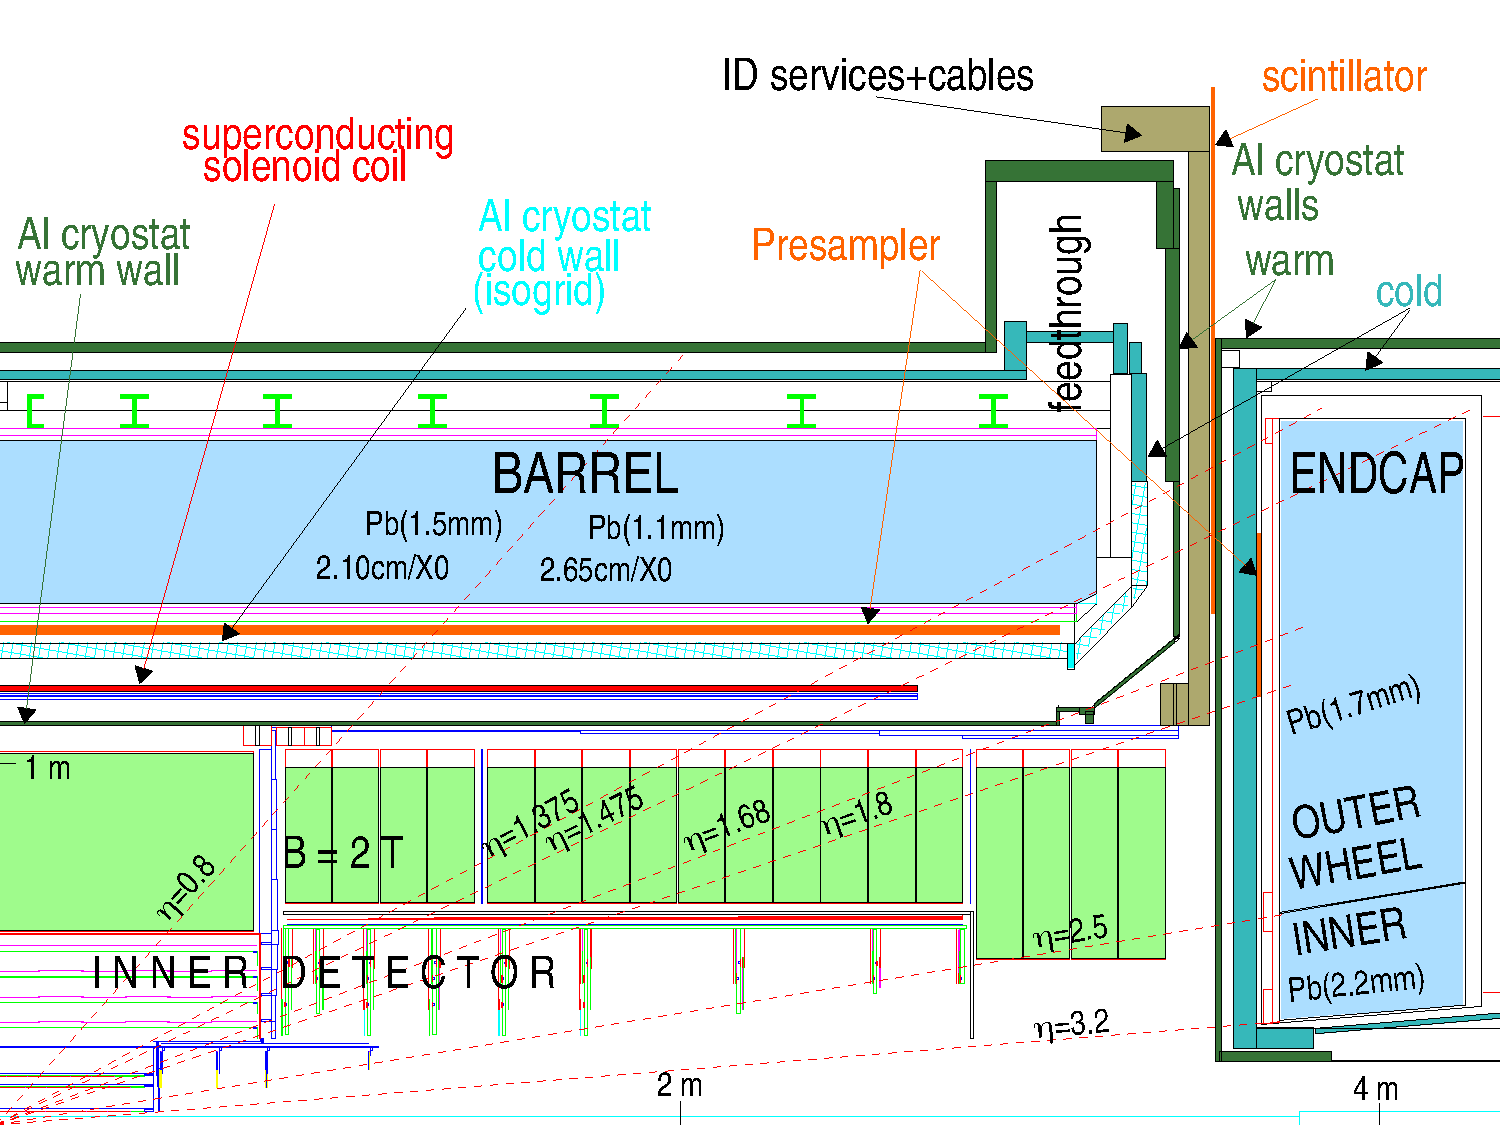
\includegraphics[width=1\textwidth]{figures/calorimetros_secao.pdf}
\caption[Seção de corte longitudinal do ECAL]
{Seção de corte longitudinal do ECAL. Extraído de
\cite{cal_tdr}}
\label{fig:secao_em_calo}
%\end{sidewaysfigure}
\end{figure}
%\end{landscape}


\begin{table}[p]\scriptsize
\centering 
\resizebox{\textwidth}{!}{
\begin{tabular}{p{5cm} c c c}
  \hline
  \hline
  \textbf{Pré-amostrador (PS)}    & \textbf{Barril}  & \textbf{Tampa} &  \\  \hline
  Cobertura   &  $|\eta|<1,52$ & $1,5<|\eta|<1,8$   \\
  Segmentação Longitudinal & 1 camada  & 1 camada  \\
  Granularidade ($\Delta \eta \times \Delta \phi$)    &  $0,025 \times 0,1$ &
$0,025 \times 0,1$  \\
  Canais de Leitura & 7808 & 1536 (ambos os lados)\\
  \hline
  \hline
  \textbf{Eletromagnético}    & \textbf{Barril}  & \textbf{Tampa (EMEC)}  \\  \hline
  Cobertura   &  $|\eta|<1,475$ & $1,375<|\eta|<3,2$   \\
  Segmentação Longitudinal & 3 camadas  & 3 camadas & $1,5   < |\gls{eta}| < 2,5$ \\
  & & 2 camadas & $1,375   < |\gls{eta}| < 1,5$ \\
  & & 2 camadas & $2,5     < |\gls{eta}| < 3,2$ \\
  Granularidade ($\Delta \eta \times \Delta \phi$)& &  \\
  Camada 1  & $0,003 \times 0,1 $  & $0.025 \times 0.1$ & $1,375 < |\gls{eta}| <
1,5$ \\ 
            &                      & $0,003 \times 0,1$ & $1,5   < |\gls{eta}| <
1,8$ \\
            &                      & $0,004 \times 0,1$ & $1,8   < |\gls{eta}| <
2,0$ \\
            &                      & $0,006 \times 0,1$ & $2,0   < |\gls{eta}| <
2,5$ \\
            &                      & $0,1   \times 0,1$ & $2,5   < |\gls{eta}| <
3,2$ \\

  Camada 2  & $0,025 \times 0,025$ & $0,025 \times 0,025$   & $1,375 <
|\gls{eta}| < 2,5$ \\
            &                      & $0,1 \times 0,1$      & $2,5   <
|\gls{eta}| < 3,2$ \\
  Camada 3  & $0,050 \times 0,025$ & $0,050 \times 0,025$  & $1,5   <
|\gls{eta}| < 2,5$ \\
  Canais de Leitura & 101760 & 62208 (ambos os lados)\\
   \hline
   \hline
  \textbf{Had. Telhas Cintilantes (\emph{TileCal})}    & \textbf{Barril}  & \textbf{Barril
estendido}     \\  \hline
  Cobertura   &  $|\eta|<1,0$ & $0,8<|\eta|<1,7$   \\
  Segmentação Longitudinal & 3 camadas  & 3 camadas  \\
  Granularidade ($\Delta \eta \times \Delta \phi$)& &  \\
  Camadas 1, e 2    &  $0,1 \times 0,1$ & $0,1 \times 0,1$   \\
  Camada 3   &  $0,2 \times 0,1$ & $0,2 \times 0,1$   \\
  Canais de Leitura & 5760 & 4092 (ambos os lados)\\
  \hline
  \hline
  \textbf{Had. Argônio Líquido (HEC)}    &  &  \textbf{Tampa}     \\  \hline
  Cobertura   &   & $1,5<|\eta|<3,2$  \\
  Segmentação Longitudinal &   & 4 camadas  \\
  Granularidade ($\Delta \eta \times \Delta \phi$)& & $0,1 \times 0,1 $ & $1,5 <
|\gls{eta}| < 2,5$ \\
  & & $0,2 \times 0,2 $ & $ 2,5 < |\gls{eta}| < 3,2$ \\
  Canais de Leitura & & 5632 (ambos os lados)\\
  \hline
  \hline
  \textbf{Calorímetro Dianteiro (FCal)}    &  &   \textbf{Dianteiro}    \\  \hline
  Cobertura   &  & $ 3,1 < |\gls{eta}| < 4,9 $ \\
  Segmentação Longitudinal &   & 3 camadas  \\
  Granularidade ($\Delta \eta \times \Delta \phi$)& & $\sim0,2 \times 0,2$  \\
  Canais de Leitura & & 1762 (ambos os lados)\\
  \hline
  \hline
\end{tabular}
}
\caption[Região de cobertura em $\eta$, granularidade e
número de canais de leitura das camadas dos calorímetros]
{Região de cobertura em $\eta$, granularidade e
número de canais de leitura das camadas dos calorímetros. Adaptado de
\cite{tese_eduardo}}
\vspace{.3cm}
\label{tab:calo}
\end{table}



Um corte longitudinal do \gls{ecal} está disposto na
Figura~\ref{fig:secao_em_calo}. Devido a complexidade da geometria do
calorímetro, existem três regiões de fissuras, também simétricas em \gls{phi}, 
nas quais a resposta do detector é degradada em comparação com o resto 
da cobertura. São elas:

\begin{itemize}
\item $\gls{eta}=0$ : entre a junção das duas metades do barril, existe uma 
pequena fissura totalizando 6~mm de \gls{lar} inativo;
\item $|\gls{eta}|\sim1,45$ : a região de transição entre o barril e a tampa é
utilizada como trajeto para os cabos e serviços do \gls{id}. Essa região é a
maior fissura do detector, começando a degradar lentamente a resposta do detector em
$|\gls{eta}|>1,35$, e indo até cerca de $|\gls{eta}|<1,68$;
\item $|\gls{eta}|=2,5$ : na região de transição entre a tampa mais externa e
interna do detector uma pequena fissura de 3~mm. Uma degradação adicional é
causada por um material morto colocado na frente deste local como um anel de
suporte.
\end{itemize}

A estrutura de acordeão
tem como vantagem a flexibilidade de segmentação longitudinal e transversa,
permitindo a implementação de camadas com diferentes granularidades. São
utilizadas três camadas, que podem ser observadas na
Figura~\ref{fig:cal_lar_camadas}, com as seguintes propriedades:

\begin{figure}[h!t]
\centering
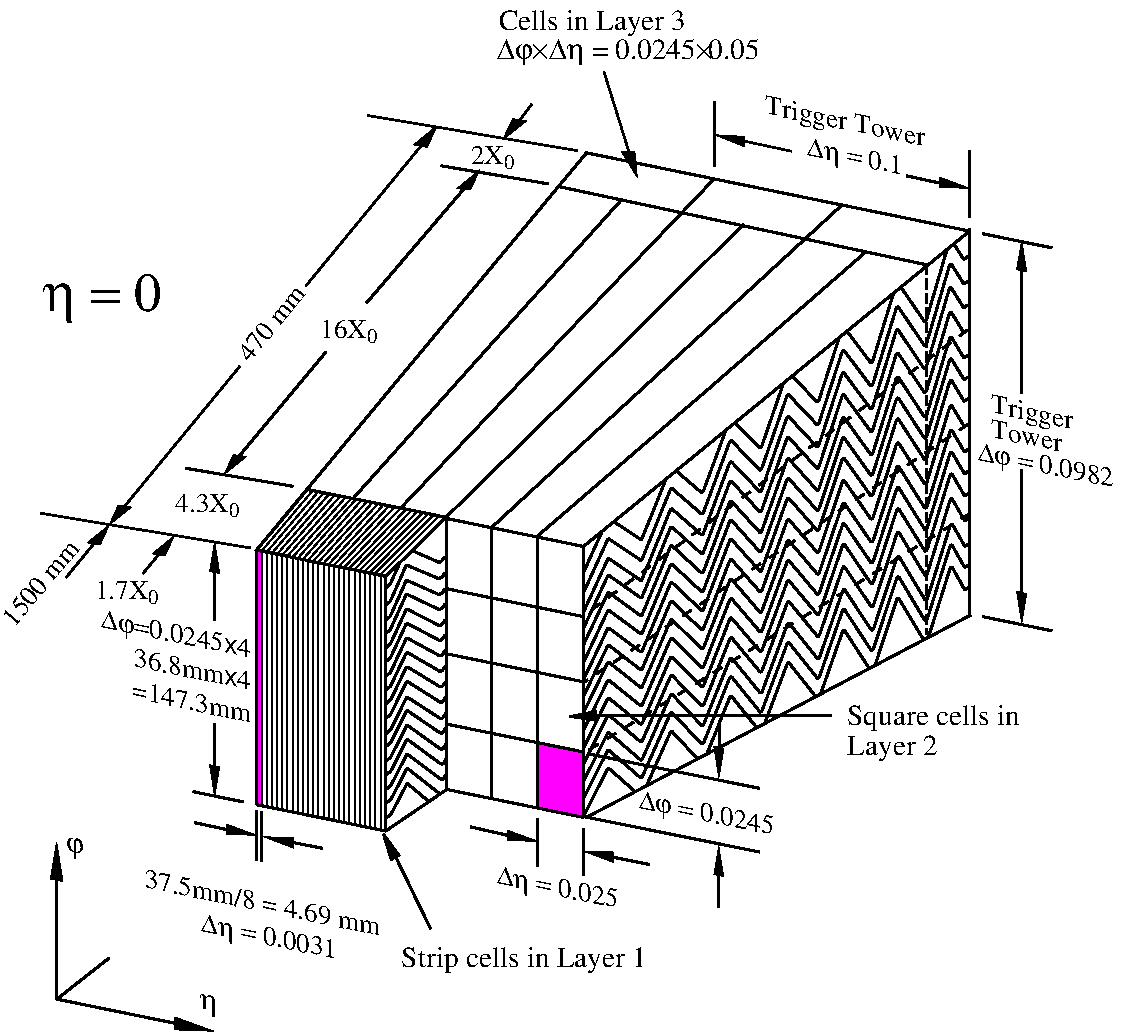
\includegraphics[width=.6\textwidth]{figures/cal_lar_camadas.pdf}
\caption[Esboço da estrutura do acordeão e a granularidade de suas camadas para
o EMB]{Esboço da estrutura de acordeão e a granularidade de suas camadas para
$|\eta|=0$ do EMB. A quantidade de $X_0$ típicos para cada uma das camadas também é
mostrada. Extraído de \cite{cal_tdr}.}
\label{fig:cal_lar_camadas}
\end{figure}

\begin{itemize}
\item \textbf{\gls{e1}}: a primeira camada é composta por tiras
finas com grande granularidade em \gls{eta}, tendo como objetivo fazer uma
boa leitura dessa posição. Isso é especialmente importante no caso de fótons,
que não são medidos pelo detector de traços, e ao mesmo tempo para casar os
traços das partículas com seus respectivos chuveiros. Conforme o \gls{eta} aumenta,
há um decréscimo da granularidade devido ao fato das tiras não poderem ser feitas com menos de 5~mm.
A escolha de tiras mais grosseiras em \gls{phi} quando comparadas com a segunda e 
terceira camadas é consequência do campo magnético do \gls{cs} espalhar os
chuveiros em \gls{phi} que possam ocorrer antes do calorímetro.


\item \textbf{\gls{e2}}: a segunda camada é responsável pela
absorção da maior quantidade de energia. Ela é segmentada transversalmente em
torres quadradas de $(\Delta\eta\times\Delta\phi)\approx(0,025\times0,025)$, que
permitem um compromisso ótimo entre a contenção do perfil lateral do chuveiro
com a contribuição do ruído por Empilhamento e eletrônico para a medição de
energia.

\item \textbf{\gls{e3}}: a terceira camada tem a mesma
granularidade que a central em \gls{phi}, mas sua granularidade é duas vezes mais grosseira
em \gls{eta}. Ela é utilizada para separar chuveiros de altas energias, e
contribui para a separação de $\gamma/$jato e elétron/jato. No caso da tampa
para $|\gls{eta}|>2,5$ são utilizadas apenas duas camadas com granularidade mais
grosseira, uma vez que se está fora da região de precisão.
\end{itemize}

Para fazer a medição com precisão da energia é necessário o mínimo de material 
antes de sua medição, de modo que essa não seja prejudicada pela geração de
chuveiros antes dos calorímetros, o que causaria a perda de energia das
partículas e deteriorando, simultaneamente, a precisão da posição de impacto 
da partícula com o mesmo. Por mais que todo o material colocado antes do
calorímetro tenha sido otimizado para minimizar esse efeito, ainda assim é
possível que isso ocorra, de modo que um instrumento Pré-amostrador foi colocado 
para estimar a perda de energia no material existente antes do calorímetro, 
estando descrito no Subtópico~\ref{par:cal_ps}.



\begin{figure}[ht!]

    \begin{center}
    
        \subfigure[Valores de $X_0$ em função de $\eta$ para as diferentes camadas do ECAL e outros materiais dispostos antes do mesmo.]
         {
            \label{fig:cal_em_x0}
            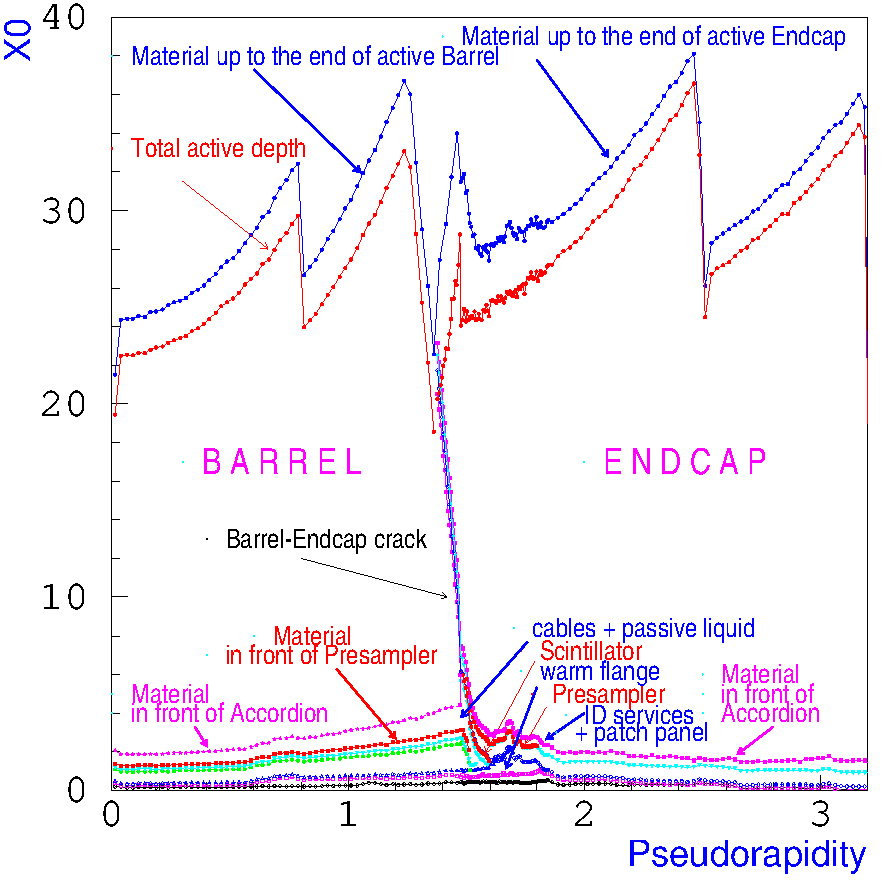
\includegraphics[width=0.46\textwidth]{figures/cal_em_x0.pdf}
        }\hspace{0.02\textwidth}
        \subfigure[Valores de $\lambda_{int}$ em função de $\eta$ para as diferentes camadas e subsistemas do calorímetro]
        {
            \label{fig:cal_had_lambda}
            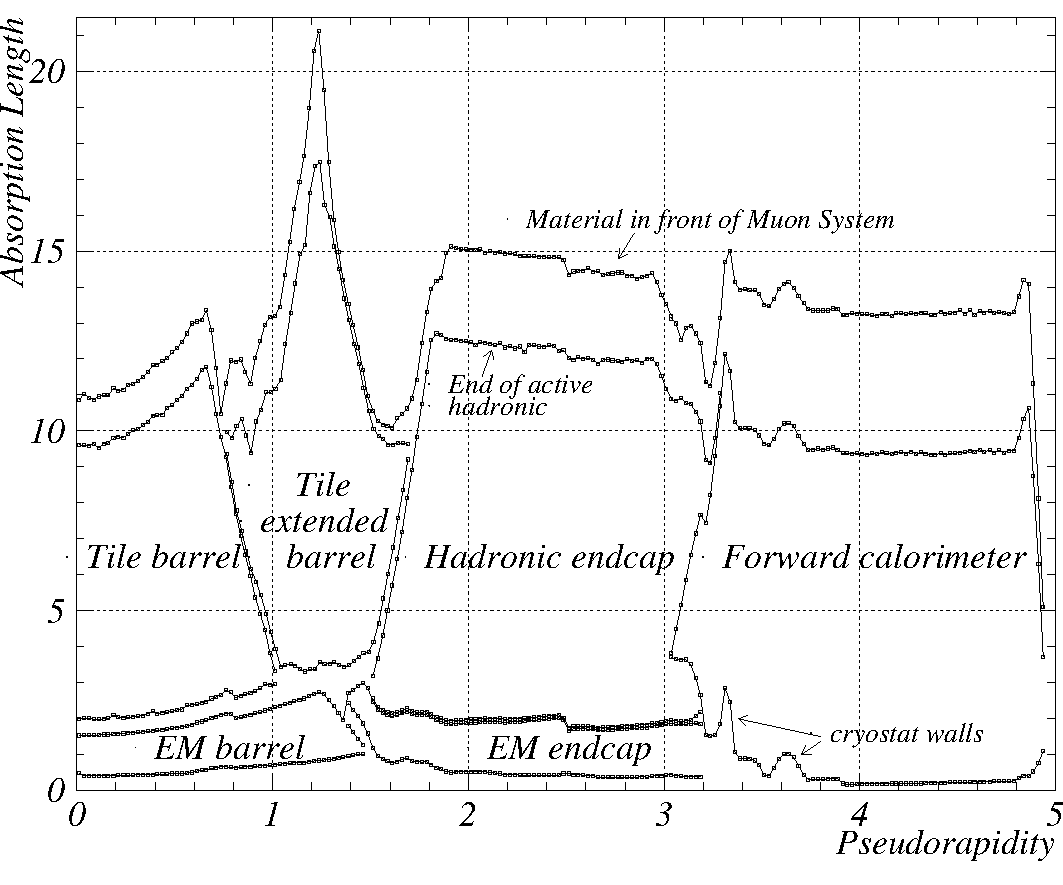
\includegraphics[width=0.46\textwidth]{figures/cal_had_lambda.pdf}
        }\\ 

    \end{center}
    
    \caption[Valores de $X_0$ e $\lambda_{int}$ em função de $\eta$ para as diferentes camadas e subsistemas.]
    {Valores de $X_0$ e $\lambda_{int}$ em função de $\eta$ para as diferentes
camadas e subsistemas. Extraído de \cite{cal_tdr}.}

\end{figure}


O \gls{ecal} tem de ser capaz de absorver completamente a energia
das partículas que devem variar de 50~MeV até 3~TeV. 
Para absorver as partículas com maiores energias, o \gls{ecal} conta com valores
maiores a 24~\gls{X0} no barril, e maiores a 26~\gls{X0} na tampa. Os valores de \gls{X0} em 
função de \gls{eta} estão dispostos na Figura~\ref{fig:cal_em_x0}, onde também é possível
visualizar os valores desse parâmetro para os materiais localizados antes do
calorímetro.

\subsubsection{Calorímetro Hadrônico de Telhas (\emph{TileCal})}
\label{par:cal_tilecal}

No barril do \gls{hcal}, chamado de \gls{tilecal}, o meio de amostragem consiste de telhas de
cintiladores de plástico e seu material passivo é o aço (o \gls{lambdaint} é
aproximadamente igual ao do chumbo, cerca de $16,8$~cm\fnref{fn:comp_rad_nucl}), Figura~\ref{fig:estr_tilecal}. 
Ao invés do efeito capacitivo utilizado no \gls{lar}, os cintiladores de
plástico são excitados pelas partículas carregadas do chuveiro, de modo que são
emitidos fótons capturados por fibras óticas, que os direcionam aos
\glspl{pmt}. Os \glspl{pmt} geram um sinal proporcional a energia da partícula
que iniciou o chuveiro.
Essa técnica de amostragem é utilizada pois nesta região mais externa e central do detector 
há pouca incidência de radiação\footnote{Uma relação entre a incidência de
radiação e pseudorrapidez foi feita em Seção~\ref{ssec:det_int}.\label{fn:radiacao}}, 
sendo possível utilizar um método com menor custo financeiro.

O \gls{tilecal} é segmentado longitudinalmente para garantir melhor identificação
das partículas, e pela possibilidade de conseguir uma melhor resolução de
energia através da calibração realizada pela ponderação do depósito em cada um
das camadas. São utilizadas três camadas para esse propósito: \gls{h0}, \gls{h1} 
e \gls{h2}.

A resolução de energia do calorímetro necessária para fazer a medição dos
diversos jatos e hádrons gerados nas colisões e dos jatos duplos provenientes 
dos decaimentos do bóson W tem de atender \ref{eq:res_tile1}. 
A linearidade de resposta do calorímetro mínima é de 2\% em uma escala de até 4
GeV.

\begin{equation}\label{eq:res_tile1}
\frac{\delta E}{E} \approx \frac{50\%}{\sqrt{E}} \oplus 3\% \;\ \text{para} \;\
|\gls{eta}|<3
\end{equation}

É necessário que o \gls{hcal} tenha no mínimo a espessura de 10 \gls{lambdaint}
para a contenção completa dos chuveiros, tanto para garantir resolução de
energia, quanto reduzir o ruído causado no Espectrômetro de Múons. Os valores de
\gls{lambdaint} para os diversos \gls{hcal} estão dispostos na
Figura~\ref{fig:cal_had_lambda}.


\subsubsection{Tampas do Calorímetro Hadrônico (HEC)}
\label{par:cal_hec}

Para a \gls{hec} também se utiliza o \gls{lar} como meio ativo devido a
incidência de radiação, mas ao invés de chumbo, seu material passivo é o cobre
($\gls{X0} = 1,43$~cm e $\gls{lambdaint}=9,39$~cm\fnref{fn:comp_rad_nucl}). 
Sua estrutura foi projetada como uma chapa plana 
demonstrada na Figura~\ref{fig:estr_hec}. São utilizadas duas tampas para cada
\gls{hec} contendo cada uma 32 módulos idênticos. Cada módulo consiste de 24
chapas de cobre para a primeira tampa, e 16 chapas para a segunda. Em ambos os
casos as chapas de cobre estão separadas por uma fissura de 8,5~mm contendo
\gls{lar} e três eletrodos. Essa estrutura foi escolhida principalmente por ter
uma maior resistência a radiação e eficácia de custo, ainda fornecendo a
cobertura espacial necessária.

Os requisitos de linearidade e de resolução de energia devem atender aqueles
especificados para o \gls{tilecal}. Ainda, um tempo de pico de sinal
de $\sim40$ ns deve ser atendido pelo \gls{lar}. O número de \gls{lambdaint} da
\gls{hec} em função de $\gls{eta}$ estão na Figura~\ref{fig:cal_had_lambda}.

Diferente do barril, a tampa do \gls{hec}
possui 4 camadas, mas normalmente as duas camadas centrais são agrupadas em uma
única camada, de forma a manter a uniformidade de segmentação longitudinal do
\gls{hcal}.

\subsubsection{Calorímetro Dianteiro (FCal)}
\label{par:cal_fcal}

Já o \gls{fcal} apresenta uma estrutura diferenciada
para aguentar os elevados índices de radiação próximos ao tubo do feixe. Em sua primeira camada, 
é utilizada uma matriz de metal absorvedora de cobre contendo buracos igualmente
distribuídos. Nesses buracos são colocados uma estrutura de hastes coaxiais e tubos, 
ambos novamente de cobre, separados por um preciso pedaço de fibra de plástico resistente
a radiação. A matriz e o tubo compõem o material passivo,
enquanto o espaço remanescente entre o tubo e a haste é preenchido por \gls{lar},
o meio de amostragem. O tubo está aterrado, enquanto as hastes estão em alta tensão, 
criando o efeito capacitivo.
Essa estrutura fica mais facilmente compreendida na Figura~\ref{fig:estr_fcal}. 
O material das hastes e da matriz são substituídos de cobre para tungstênio
($\gls{X0} = 0,350$~cm e $\gls{lambdaint} = 5,72$~cm\fnref{fn:comp_rad_nucl}) com 
o objetivo de elevar a capacidade de absorção de partículas \gls{had} nas segunda 
e terceira camadas. O acumulo de íons de \gls{lar} nas fissuras limita a
luminosidade máxima proporcionalmente a $1/g^2$, de forma que o comprimento das
fissuras (g) devem ser os menores possíveis. 
As dimensões das mesmas são de 250-375~$\mu$m para a seção \gls{em} 
e 500~$\mu$m para a seção \gls{had}.


A tarefa principal desse detector é a reconstrução de jatos e fornecer
hermeticidade para a medição de \gls{ptmiss}. Por isso, a resolução de energia para 
o \gls{hcal} na região dianteira pode ser menor, de
acordo com a Equação~\ref{eq:res_tile2}. Nessa região, também, é necessária a identificação de
jatos dianteiros uma vez que a região de admissão para seus decaimentos do
bóson de Higgs é de $2<|\gls{eta}|<5$. Observe novamente a
Figura~\ref{fig:cal_had_lambda} para os comprimentos do \gls{fcal}.

\begin{equation}\label{eq:res_tile2}
\frac{\delta E}{E} \approx \frac{100\%}{\sqrt{E}} \oplus 10\% \;\ \text{para} \;\
3<|\gls{eta}|<5
\end{equation}



\begin{figure}[ht!]
    \label{fig:estruturas_cal}
    \begin{center}

        \subfigure[Acordeão para o barril do ECAL. Extraído de \cite{cal_tdr}.]{
            \label{fig:estr_acordeao}
            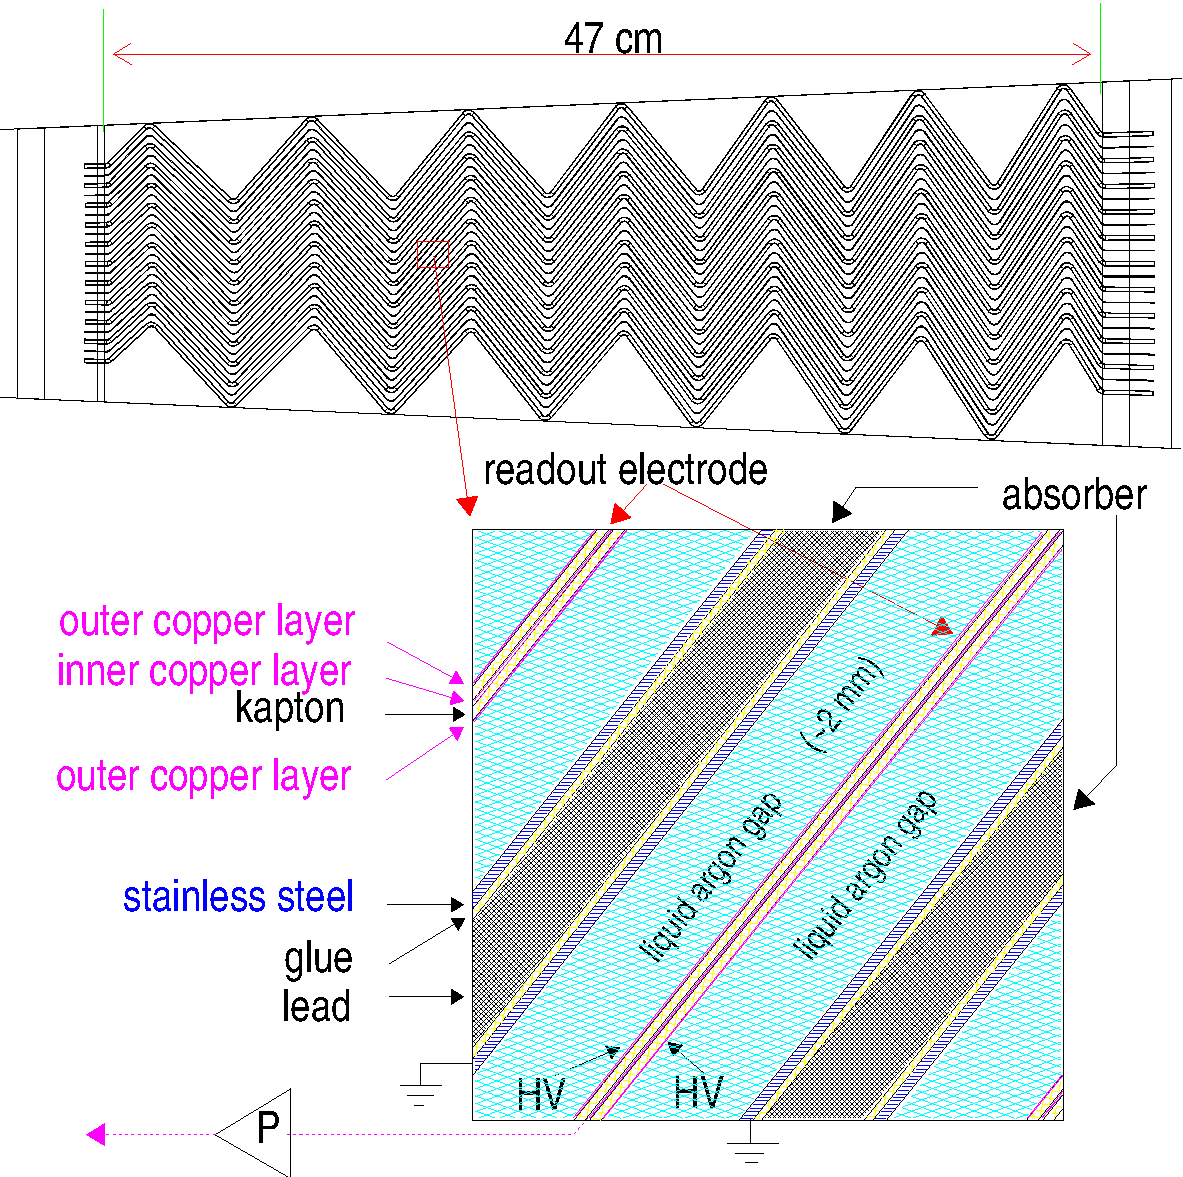
\includegraphics[width=.46\textwidth]{figures/estrutura_acordeao_barril.pdf}
        } \hspace{0.01\textwidth}
        \subfigure[Telhas e cintiladores do TileCal. Extraído de \cite{cal_tdr}]{
            \label{fig:estr_tilecal}
            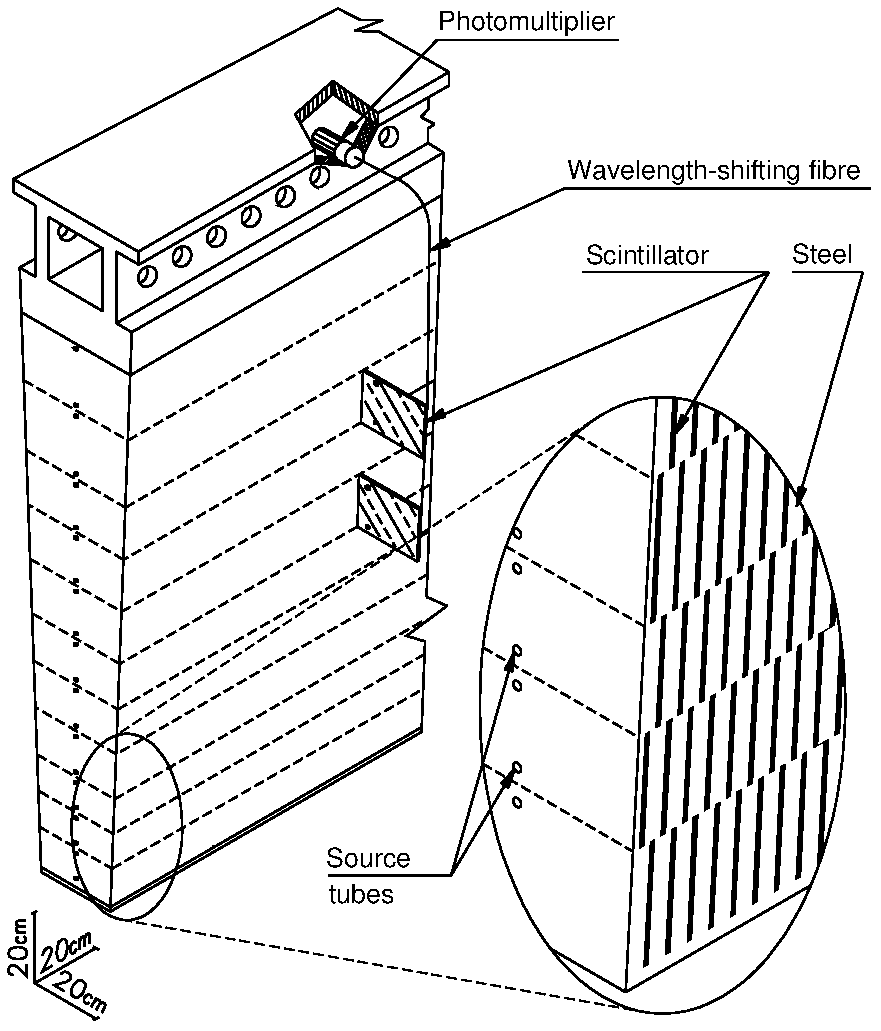
\includegraphics[width=0.46\textwidth,height=7cm]{figures/estrutura_tilecal.pdf}
        } \\
        
        \subfigure[Chapa plana do HEC. Extraído de \cite{paper_atlas}.]{
            \label{fig:estr_hec}
            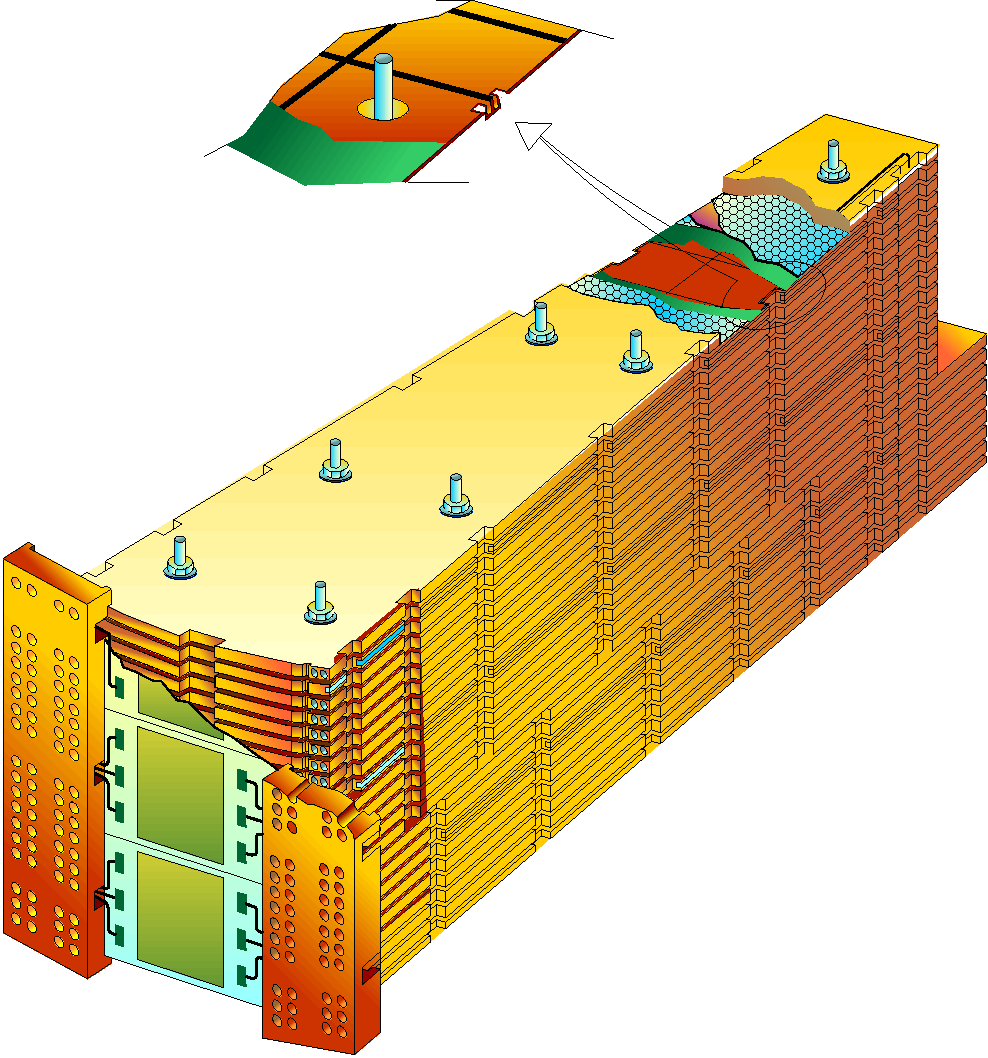
\includegraphics[width=0.46\textwidth]{figures/estrutura_hec.pdf}
        }\hspace{0.01\textwidth}
        \subfigure[Tubos e Hastes para a primeira camada do FCal. Extraído de \cite{paper_atlas}.]{
            \label{fig:estr_fcal}
            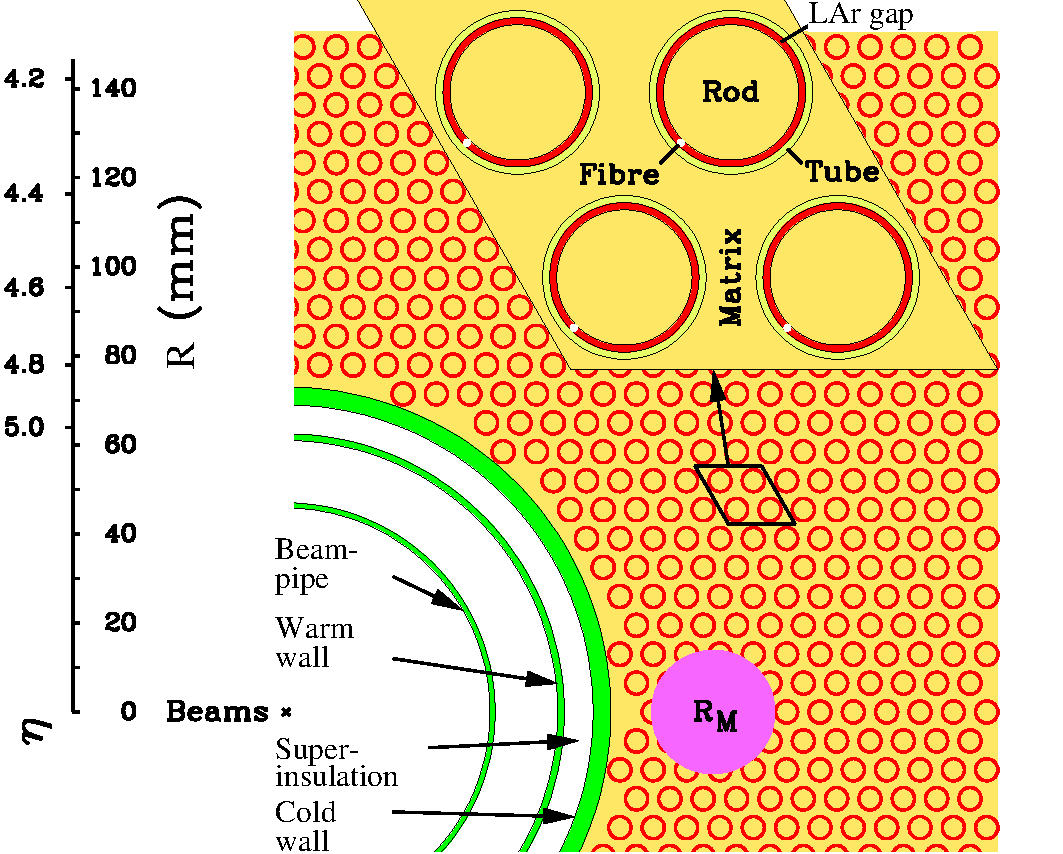
\includegraphics[width=0.46\textwidth]{figures/estrutura_fcal.pdf}
        } \\
        
    \end{center}
    \caption[As diferentes estruturas dos subsistemas de calorimetria do ATLAS]{As diferentes estruturas dos subsistemas de calorimetria do ATLAS.}
    
\end{figure}


\subsubsection{Calorímetro Pré-amostrador (PS) e Cintiladores}
\label{par:cal_ps}

O \gls{ps}, diferente dos calorímetros detalhados anteriormente, não possui meio passivo, 
constituído apenas de uma fina camada de \gls{lar} na região de
$|\gls{eta}|<1,8$. Seu barril ($|\gls{eta}|<1,52$) contém eletrodos
perpendiculares ao feixe e um comprimento de~1,1 cm, enquanto na tampa,
$1,5<|\gls{eta}|<1,8$, a configuração dos eletrodos é paralela e o comprimento
de 0,5~cm. Sua função é absorver partículas de chuveiros formados antes do
calorímetro do \gls{atlas} pela interação das partículas com o material anterior
ao calorímetro (observe os valores de \gls{X0} desses materiais na Figura~\ref{fig:cal_em_x0}), 
como no \gls{cs}, criostato e no \gls{id}. Com isso é possível realizar 
a calibração da energia perdida pelas partículas nesse material.
Além da pseudorrapidez de 1,8, o \gls{ps} não é mais 
necessário dado que o material morto (material que não contribui para a detecção
de energia da partícula) é reduzido e a energia total das partículas 
é grande para um dado \gls{pt}.

Na região de transição entre o barril e a tampa, para
$|\gls{eta}| = 1,4$, a situação é particularmente critica devido aos serviços e
cabos para o \gls{id}, e uma camada cintiladora em $1,0<|\gls{eta}|<1,6$ 
é colocada entre os dois criostatos com o objetivo de recuperar parte 
da energia perdida, principalmente por
partículas \gls{had}, mas também ajuda a reconstruir a energia de elétrons e
fótons. As disposições desses dois calorímetros, assim como do cintilador pode 
ser observada na Figura~\ref{fig:secao_em_calo}. 

\newpage
\subsection{O Espectrômetro de Múons}
\label{ssec:espectometro_muons}

Os múons como estados finais são muito importantes em diversas análises e provêm
assinaturas físicas robustas no \gls{lhc}. 
Eles penetram grandes quantidades de material enquando a maioria das outras
partículas são absorvidas, e com o objetivo de medir sua energia, o Espectrômetro
de Múons \cite{muon_tdr} é o subdetector mais externo do \gls{atlas}. Diferente dos calorímetros
que empregam um processo de medição destrutivo, o Espectrômetro de Múons,
Figura~\ref{fig:espec_muons}, mede a carga e o momento de múons através 
da reconstrução de suas trajetórias no 
campo magnético dos toroides de núcleo a ar de forma semelhante ao \gls{id}. 

\begin{figure}[h!t]
\centering
%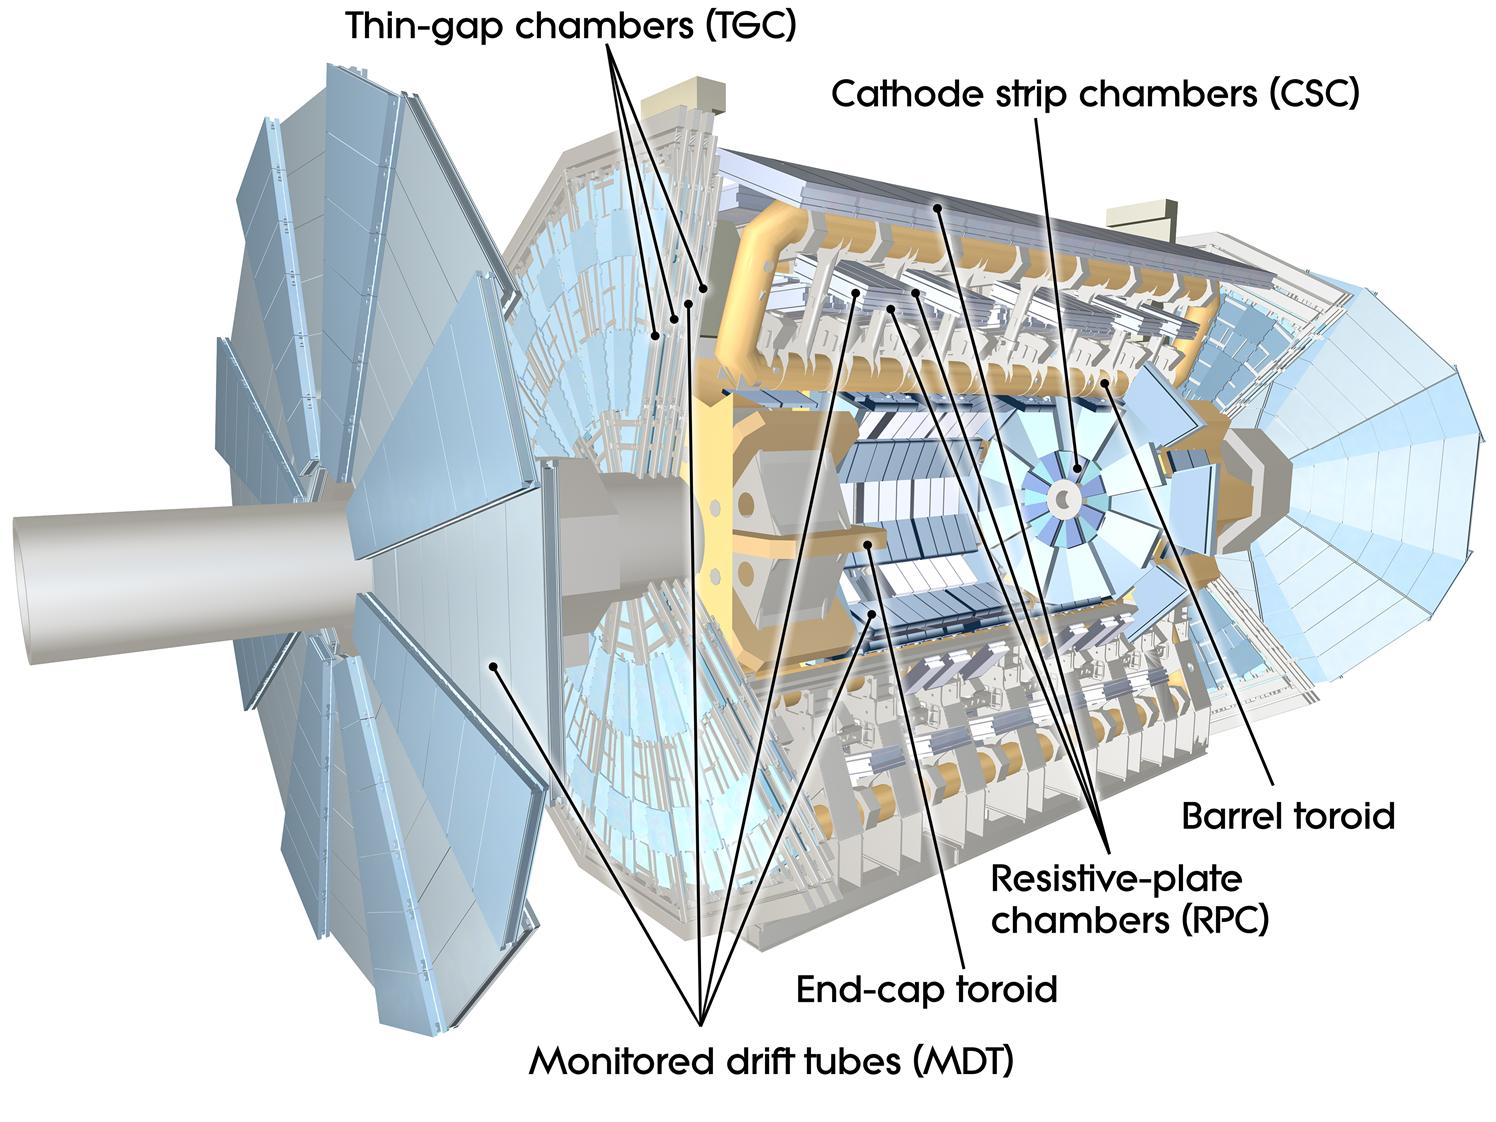
\includegraphics[width=0.8\textwidth]{imagens/espectometro_muons_lowres.jpg}
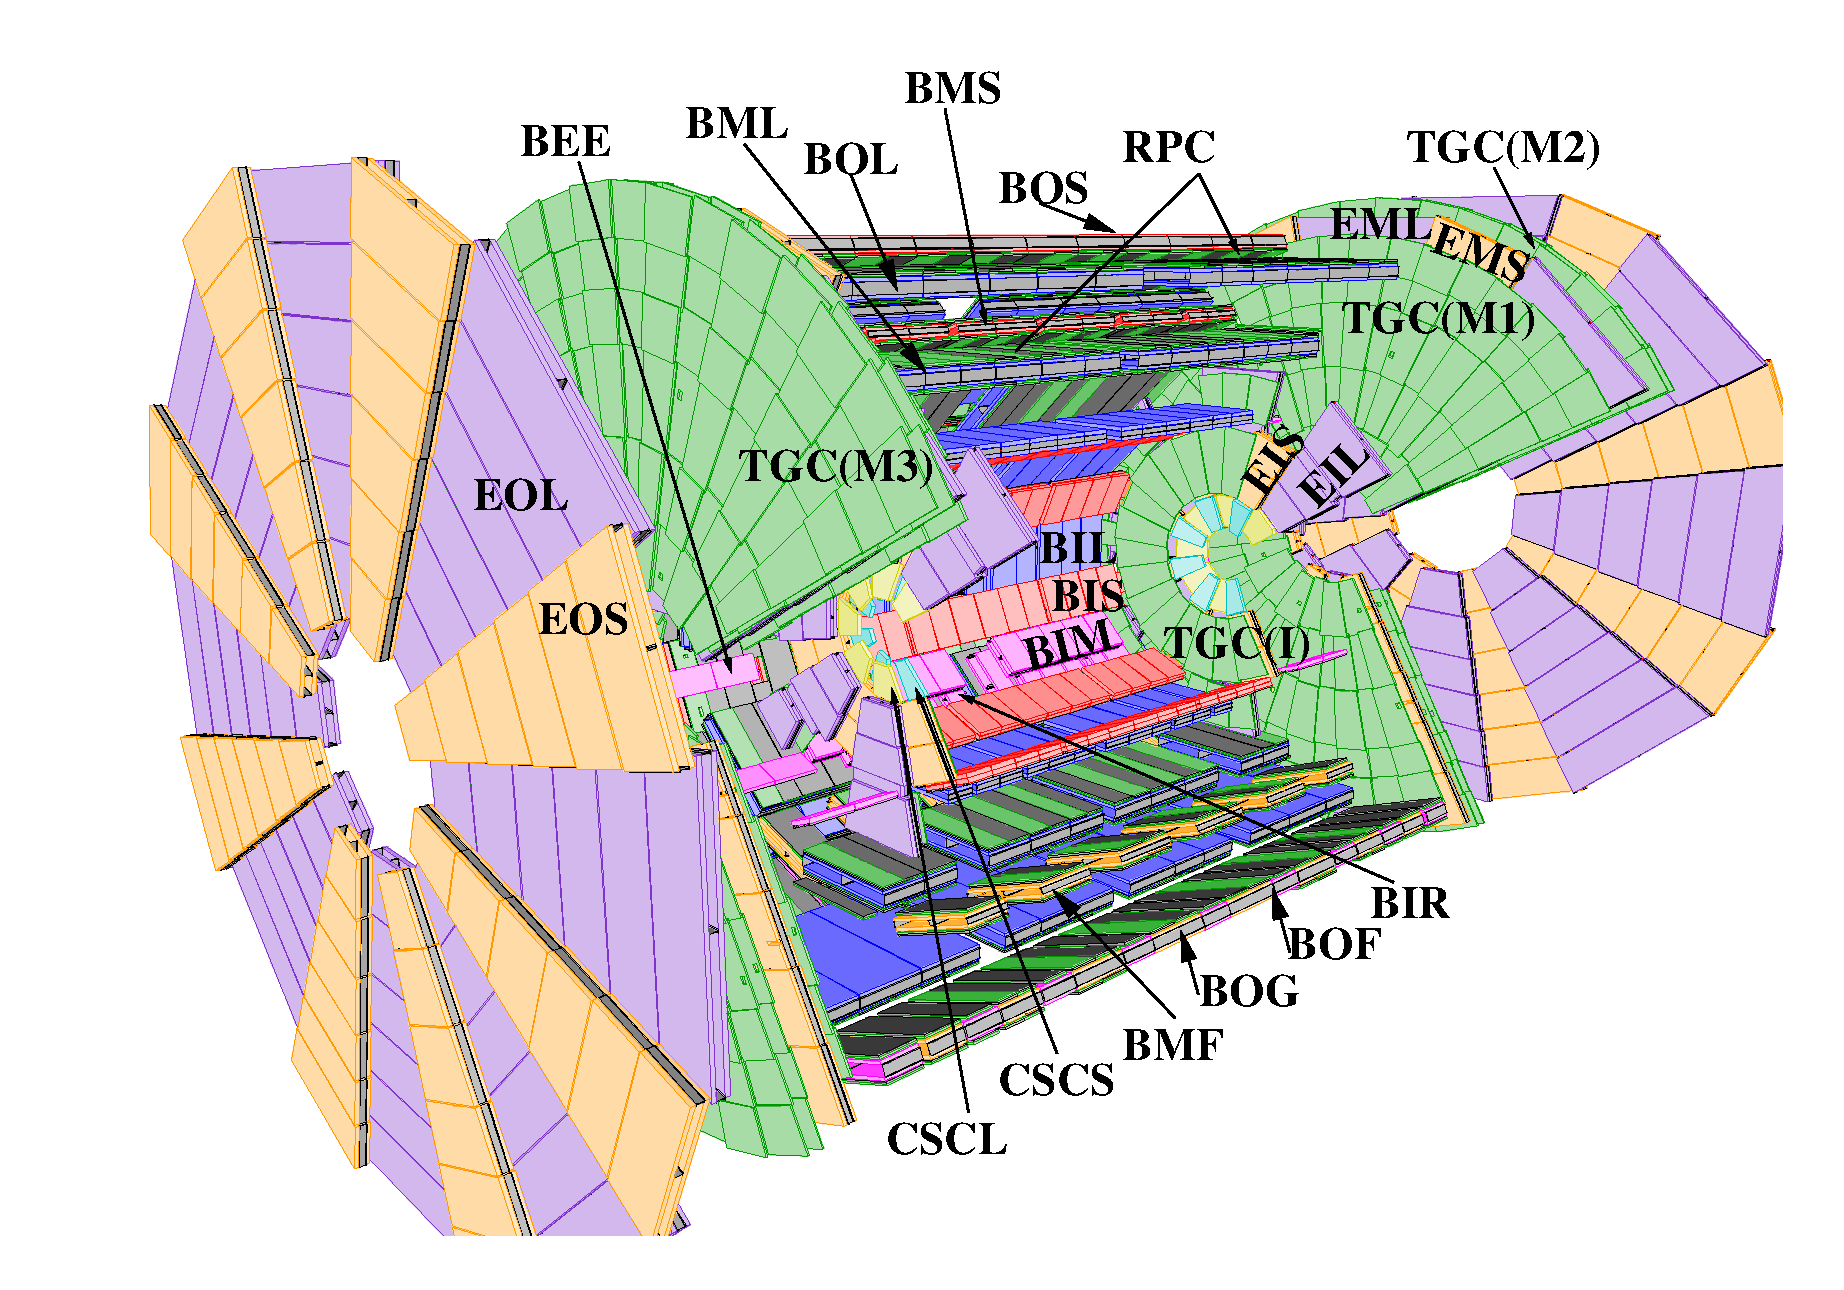
\includegraphics[width=0.7\textwidth]{figures/Muon_system_Initial.pdf}
\caption[O Espectrômetro de Múons]{
O Espectrômetro de Múons e seus subsistemas: as câmaras medidoras de
precisão: (MDTs e CSCs) e as câmaras de filtragem (RPCs e TGCs). Na tampa, a
primeira camada TGC (I) é localizada na camada mais interna; as próximas três
camadas estão na frente (M1) e atrás (M2 e M3) da segunda roda MDT. A primeira
letra (B e E) do esquema de nomenclatura do MDT faz referência às câmaras no barril
e tampa, respectivamente. A segunda e terceira letras referenciam para a camada
(interior: I, central: C, externa: O) e setor (extenso: L e pequeno: S). Extraído de
%\cite{muons_images}.}
\cite{paper_atlas}.}
\label{fig:espec_muons}
\end{figure}

As câmaras no barril formam três cilindros
concêntricos com o eixo dos feixes e cobrem um alcance em $|\gls{eta}| < 1$,
estando localizadas a uma distância radial de $\sim$5, 7,5, e 10~m. São
utilizados quatro discos para as câmaras da tampa que cobrem um o alcance de 
$1 < |\gls{eta}| < 2,7$ em distâncias de $\sim$7, 10, 14 e 21-23~m do ponto de
interação, todos concêntricos ao tubo do feixe. Deseja-se medir múons
na região de poucos GeV com uma resolução de $\sim1\%$, enquanto para múons na
faixa de 1 TeV a precisão pode ser um pouco menor ($ < 10\%$). O poder de
curvatura $Bl^2$ fornecido pelos toroides e tamanho do detector é de cerca de 36~$\text{Tm}^2$, 
comparado com os 2~$\text{Tm}^2$ no \gls{id}. Para fornecer a
resolução de momento desejada a \gls{respos} deve ser de no mínimo
50~$\mu$m em z e 0,5~mrad em R$\phi$ \cite{ATLAS_TDR}.

Existem diversos tipos de câmaras de traços de múons: As \gls{mdt} e \gls{csc}
são as câmaras de precisão, já as \gls{rpc} e \gls{tgc} são câmaras
rápidas para o \glslink{l1}{Primeiro Nível de filtragem (L1)}. O princípio de leitura é o mesmo para os quatro
tipos, onde os múons que passam por uma fenda de gás entre um anodo e catodo (por
exemplo, um cabo dentro de um tubo ou duas chapas paralelas) causam uma descarga
local no gás sendo assim possível ler o sinal. No total existem 5376 câmaras
com 1,0757~M canais de leitura \cite{tese_jatos}.

Os \glspl{mdt} fornecem medições de precisão (acurácia mecânica de 30~$\mu$m) 
dos pontos do traço com 80~$\mu$m de \gls{respos}
para cada cabo em uma larga região de \gls{eta}. Em grandes \gls{eta} e próximo
do ponto de interação são utilizados os \glspl{csc}, que têm uma maior
granularidade e suportam a sua alta demanda causada pelas condições de ruído
físico.
 
As câmaras de filtragem têm uma resolução de tempo menor que o espaçamento
mínimo entre pacotes de 25~ns para fazer possível sua identificação. Os
requisitos de tempo e espaço são atendidos de acordo com a seguinte
especificação: os \glspl{rpc} têm boa resolução de tempo (1,5~ns), por outro
lado os \glspl{tgc} tem melhor resolução espacial 
(o afastamento entre os cabos anodos é de 1,8~mm).

Graças a grande dimensão do Espectrômetro de Múon não é possível de firmar as
dimensões e posições das câmaras no nível requerido de 30~$\mu$m. Portanto, as
deformações e posições da câmara são constantemente monitoradas por meio de
sistemas ópticos de alinhamento, de forma que deslocamentos dentre $\sim$30~$\mu$m e $\sim$1~cm 
podem ser corrigidos em análise pelos algoritmos do
\glsdesc{sr} \cite{muon_tdr}.










